\documentclass[t,handout]{beamer}
\usepackage[utf8]{inputenc}
\usepackage[ngermanb]{babel}
\usepackage{listings}
\lstset{ % 
  basicstyle=\tiny,
  breaklines=true,
  frame=single
}

\definecolor{darkblue}{rgb}{0,0,.5}
\hypersetup{pdftex=true, colorlinks=true, breaklinks=true, linkcolor=darkblue, menucolor=darkblue, pagecolor=darkblue, urlcolor=darkblue}

\title{Taskwarrior -- What's next?}
\subtitle{Task management on the commandline}
\author[Deimeke, Dirk]{Dirk Deimeke}
\institute[Swiss Perl Workshop 2014]{Swiss Perl Workshop 2014}
\date{September, 05th 2014}
\titlegraphic{
\includegraphics[width=3cm,height=3cm]{tw-xxl}}
\subject{Taskwarrior}
\keywords{taskwarrior, task, management, commandline, getting things done}

\setbeamercovered{transparent}

\pgfdeclareimage[width=5mm]{tw-logo}{tw-xl}

%%%%%%%%%%%%%%%%%%%%%%%%%%%%%%%%%%%%%%%%%%%%%%%%%%%%%%%%%%%%%%%%%%%%%%%
%
% LaTeX-Template for Taskwarrior by Dominik Wagenführ
% http://www.deesaster.org/
%
% Creative Commons Attribution-ShareAlike 4.0 (CC-BY-SA 4.0)
% https://creativecommons.org/licenses/by-sa/4.0/
%
%%%%%%%%%%%%%%%%%%%%%%%%%%%%%%%%%%%%%%%%%%%%%%%%%%%%%%%%%%%%%%%%%%%%%%%

%%%%%%%%%%%%%%%%%%%%%%%%%%%
% Layout - Start
%%%%%%%%%%%%%%%%%%%%%%%%%%%

\setbeamertemplate{navigation symbols}{}

\useinnertheme{default}
\useoutertheme{infolines}
\usefonttheme{structurebold}

\newlength{\boxwidth}
\setlength{\boxwidth}{121px}
\setbeamertemplate{headline}{%
\begin{beamercolorbox}[dp=3px,ht=6px,wd=\boxwidth,center]{palette tertiary}%
\insertauthor\ (\insertinstitute)%
\end{beamercolorbox}%
\vskip-9px\hskip\boxwidth
\begin{beamercolorbox}[dp=3px,ht=6px,wd=\boxwidth,center]{palette secondary}%
\inserttitle%
\end{beamercolorbox}%
\begin{beamercolorbox}[dp=3px,ht=6px,wd=\boxwidth,right]{palette primary}%
\insertdate\hskip15px\insertframenumber\,/\,\inserttotalframenumber\hspace*{8px}
\end{beamercolorbox}%
}
\setbeamertemplate{footline}{}

%%%%%%%%%%%%%%%%%%%%%%%%%%%
% Colors - Start
%%%%%%%%%%%%%%%%%%%%%%%%%%%

\definecolor{basecolor}{gray}{0.2}
\definecolor{mittelgrau}{gray}{0.4}
\definecolor{hellgrau}{gray}{0.93}
\definecolor{gelb}{rgb}{1.0,1.0,0.75}

% infolines color
\setbeamercolor{palette primary}{fg=white,bg=mittelgrau}
\setbeamercolor{palette secondary}{fg=white,bg=basecolor}
\setbeamercolor{palette tertiary}{fg=white,bg=black}

% frame and title color
\setbeamercolor{frametitle}{fg=white,bg=basecolor}
\setbeamercolor{titlelike}{fg=white,bg=basecolor}
\setbeamerfont{frametitle}{series=\bfseries}

% TOC color
\setbeamercolor{section in toc}{fg=basecolor}

% text color
\setbeamercolor{normal text}{fg=black,bg=white}

% item color
\setbeamercolor{item}{fg=basecolor}
\setbeamercolor{itemize item}{fg=black}

% block color
\setbeamercolor{block title}{fg=black,bg=gelb}
\setbeamercolor{block body}{fg=black,bg=gelb}

% block alert color
\setbeamercolor{block title alerted}{fg=black,bg=gelb}
\setbeamercolor{block body alerted}{fg=black,bg=gelb}

% block example color
\setbeamercolor{block title example}{fg=black,bg=gelb}
\setbeamercolor{block body example}{fg=black,bg=gelb}

\setbeamertemplate{frametitle}{%
\vskip-1px%
\begin{beamercolorbox}[wd=363px,ht=20px,dp=12px]{frametitle}
\usebeamerfont{frametitle}%
\usebeamercolor{frametitle}%
\vspace*{-5px}\hspace*{10px}
\includegraphics[width=24px,height=24px]{tw-xl.png}\\
\vspace*{-20px}\hspace*{40px}\insertframetitle%
\end{beamercolorbox}
}

%%%%%%%%%%%%%%%%%%%%%%%%%%%
% Colors - Stop
%%%%%%%%%%%%%%%%%%%%%%%%%%%

%%%%%%%%%%%%%%%%%%%%%%%%%%%%%%%%%%%%%%%%%%%%%%%%%%%%%%%%%%%%%%%%%%%%%%%

\begin{document}

\begin{frame} % Titel
	\titlepage
\end{frame}

% \logo{\pgfuseimage{tw-logo}}

\begin{frame}\frametitle{Content}
	\tableofcontents
\end{frame}

%%%%%%%%%%%%%%%%%%%%%%%%%%%
\section{Introduction} 
%%%%%%%%%%%%%%%%%%%%%%%%%%%

\parskip1ex

\begin{frame}\frametitle{Dirk Deimeke (that's me)}
	Human being, Born 1968 in Wanne-Eickel, Living in Grüt (emigrated to Switzerland 2008), Married, Two dogs, One Horse, Blogger, Podcaster, Author, Speaker, Taskwarrior, Aikidoka, Linux guy, Systems Administrator, Systems Engineer, DevOps Engineer, Technical Architect, Technical Solution Engineer, Open Source Contributor

	Entry point for more \url{http://d5e.org/}
\end{frame}

\begin{frame}\frametitle{Dirk Deimeke (Taskwarrior)}
\begin{itemize}
	\item I first saw Taskwarrior at German Ubucon 2009 in a lightning talk of Federico Hernandez, one of the core developers. \pause
	\item Started to use it in the beginning of 2010. \pause
	\item Still enthusiastic about it! ;-) \pause
	\item In the middle of 2010 I joined the Taskwarrior team.
	\item \url{http://taskwarrior.org/}
	\item \url{http://d5e.org/taskwarrior} (German) own blog-articles
\end{itemize}
\end{frame}

\begin{frame}\frametitle{About this session}
\begin{itemize}
	\item \textbf{What is this all about?} \\
		This is about Taskwarrior, an efficient tool for task management. Techniques for time management are not part of this session. \pause \\
		(But we can discuss time management techniques later on).
	\item \textbf{Why are the slides in English?} \\
		Taskwarrior is an international project. \pause
	\item \textbf{Why do you install Taskwarrior from Source?} \\
		The version of Taskwarrior included in distributions like Ubuntu tends to be pretty old. Installation from source is not that difficult. I will explain it.
\end{itemize}

\begin{alertblock}{Attention!}
	\begin{itemize}
    	\item This workshop is not a lecture, I want to do this together with you.
    	\item Ask your questions if you have some!
	\end{itemize}
\end{alertblock}
\end{frame}

\begin{frame}\frametitle{Project founder: Paul Beckingham}
\pause
\begin{itemize}
	\item I started out using Gina Trapani's todo.sh, which was great, but I soon wanted features that would have been difficult to implement in a shell script, so I wrote my own. \pause
	\item It stemmed from the fact that a todo program needs to be simple to use, and unobtrusive, otherwise it's a hassle. But it can't be too simple. \pause
	\item If you go to the trouble of capturing this information, it seems wasteful not to leverage it.  So it has a lot of features, but tries to remain simple to use. \pause
	\item There are many different methodologies people use for managing their work, and taskwarrior tries to walk a line through the middle of all that, with features for all the different approaches. \pause
	\item Taskwarrior is intended to scale with the user, from very simple straightforward usage up to quite sophisticated task management.
\end{itemize}
\end{frame}

\begin{frame}\frametitle{Reasons for Taskwarrior}
Taskwarrior
\begin{itemize}
	\item is easy to learn.
	\item grows along with the work.
	\item is unbelievably powerful.
	\item is very fast.
	\item is easily extensible. 
	\item is platform independent:
	\begin{itemize}
		\item Most flavours of Unix and Linux, including Mac OS X
		\item Windows with Cygwin
		\item via SSH from my mobile
		\item \url{http://taskwarrior.org/download/\#dist}
	\end{itemize}
	\item is actively developed.
	\item can be influenced by users (feature requests).
	\item has excellent and very friendly support.
	\item \textbf{New in 2014: Taskserver}
\end{itemize}
\end{frame}

%%%%%%%%%%%%%%%%%%%%%%%%%%%
\section{Installation}
%%%%%%%%%%%%%%%%%%%%%%%%%%%

\begin{frame}[fragile]\frametitle{Installation with package management}
\textbf{All download-addresses} \\
\url{http://taskwarrior.org/download} \pause

\textbf{Since Maverick Meerkat in Universe} \\
(Unfortunately version is behind recent)
\begin{lstlisting}
$ sudo apt-get install task
\end{lstlisting} \pause
\end{frame}

\begin{frame}[fragile]\frametitle{Installation from source}
The Meta-Package \texttt{build-essential}, \texttt{uuid-dev} and \texttt{cmake} are all you need to compile. If you want to interact with the Taskserver, you need \texttt{libgnutls-dev} as well.
\begin{lstlisting}
$ sudo apt-get install build-essential cmake uuid-dev # libgnutls-dev
\end{lstlisting}
Download of recent version
\begin{lstlisting}
$ curl -O http://www.taskwarrior.org/download/task-2.3.0.tar.gz
$ # or wget http://www.taskwarrior.org/download/task-2.3.0.tar.gz
$ # or git clone https://git.tasktools.org/scm/tm/task.git task.git
\end{lstlisting}
Untar and compile
\begin{lstlisting}
$ tar xzvf task-2.3.0.tar.gz
$ cd task-2.3.0
$ # or cd task.git
$ cmake .
$ make
$ sudo make install
\end{lstlisting}
The last command installs Taskwarrior to /usr/local.
\end{frame}

\begin{frame}[fragile]\frametitle{Installation dependencies}
\begin{center} % 1316x838
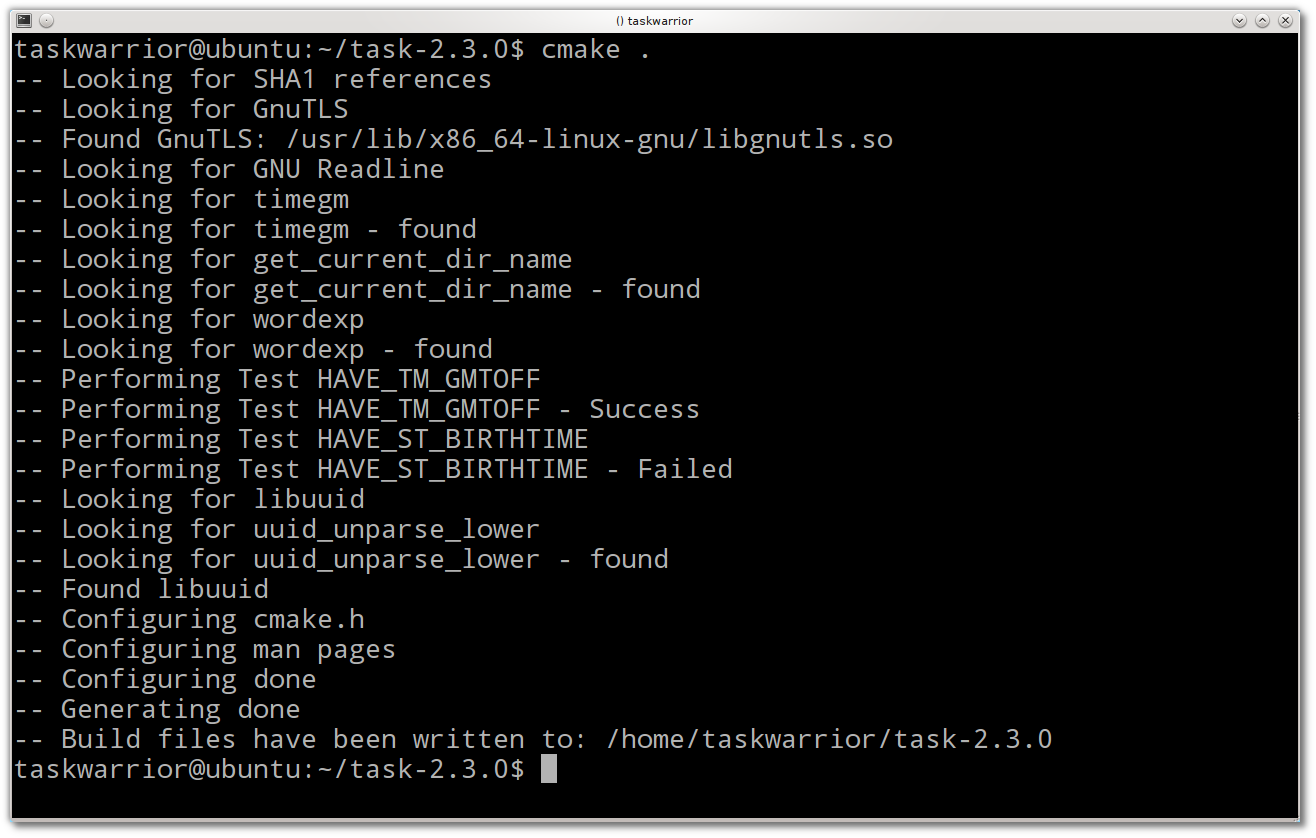
\includegraphics[width=11.8cm,height=7.5cm]{cmake.png}
\end{center}
\end{frame}

\begin{frame}[fragile]\frametitle{Installation from source with target directory}
If you don't have root permissions or in case you want to use other directories, this is possible as well. \\
(No speciality of Taskwarrior).
\begin{lstlisting}
$ cmake -DCMAKE_INSTALL_PREFIX=/home/dirk/task-2.3.0 .
$ make
$ make install # without "sudo"
\end{lstlisting}
It makes sense to define the following three variables for the next steps. (The first one is not needed, I use it only for this topic to fit on one slide).
\begin{lstlisting}
$ taskdir=/home/dirk/task_2.3.0
$ export PATH=${taskdir}/bin:${PATH}
$ export LD_LIBRARY_PATH=${taskdir}/lib:${LD_LIBRARY_PATH}
$ export MANPATH=${taskdir}/man:${MANPATH}
\end{lstlisting}
\end{frame}

\begin{frame}[fragile]\frametitle{Test of your installation}
\begin{center} % 1316x838
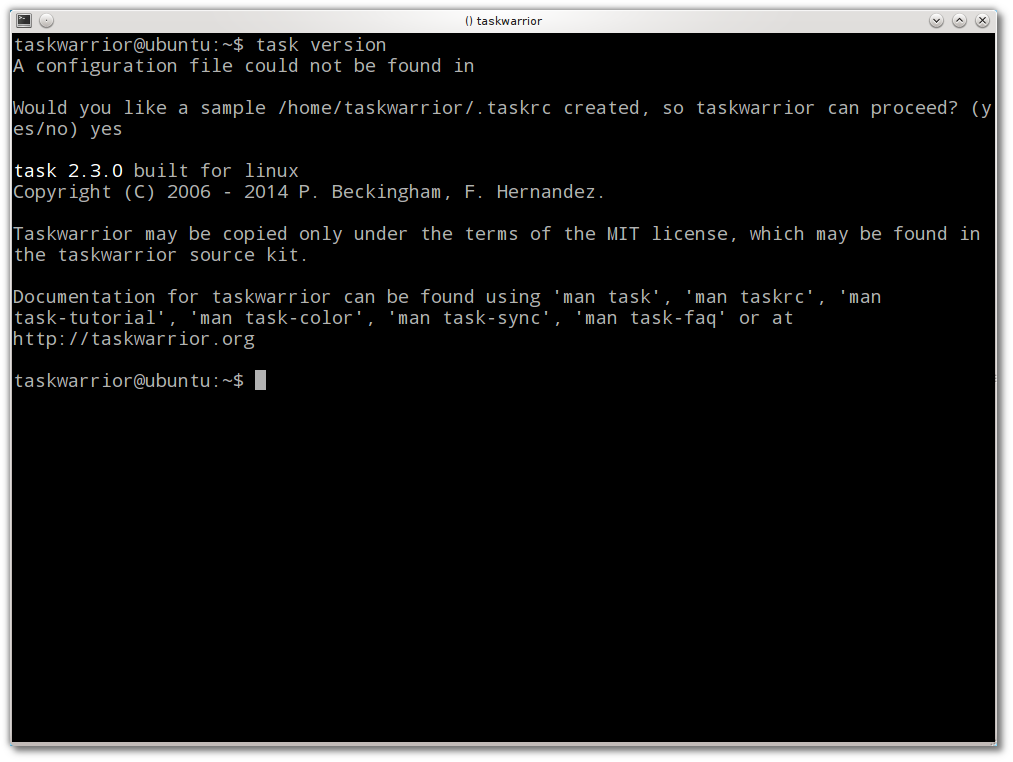
\includegraphics[width=11.8cm,height=7.5cm]{task-version.png}
\end{center}
\end{frame}

%%%%%%%%%%%%%%%%%%%%%%%%%%%
\section{Simple ToDo-Lists}
%%%%%%%%%%%%%%%%%%%%%%%%%%%

\begin{frame}[fragile]\frametitle{A simple example, part 1}
\begin{center} % 1316x838
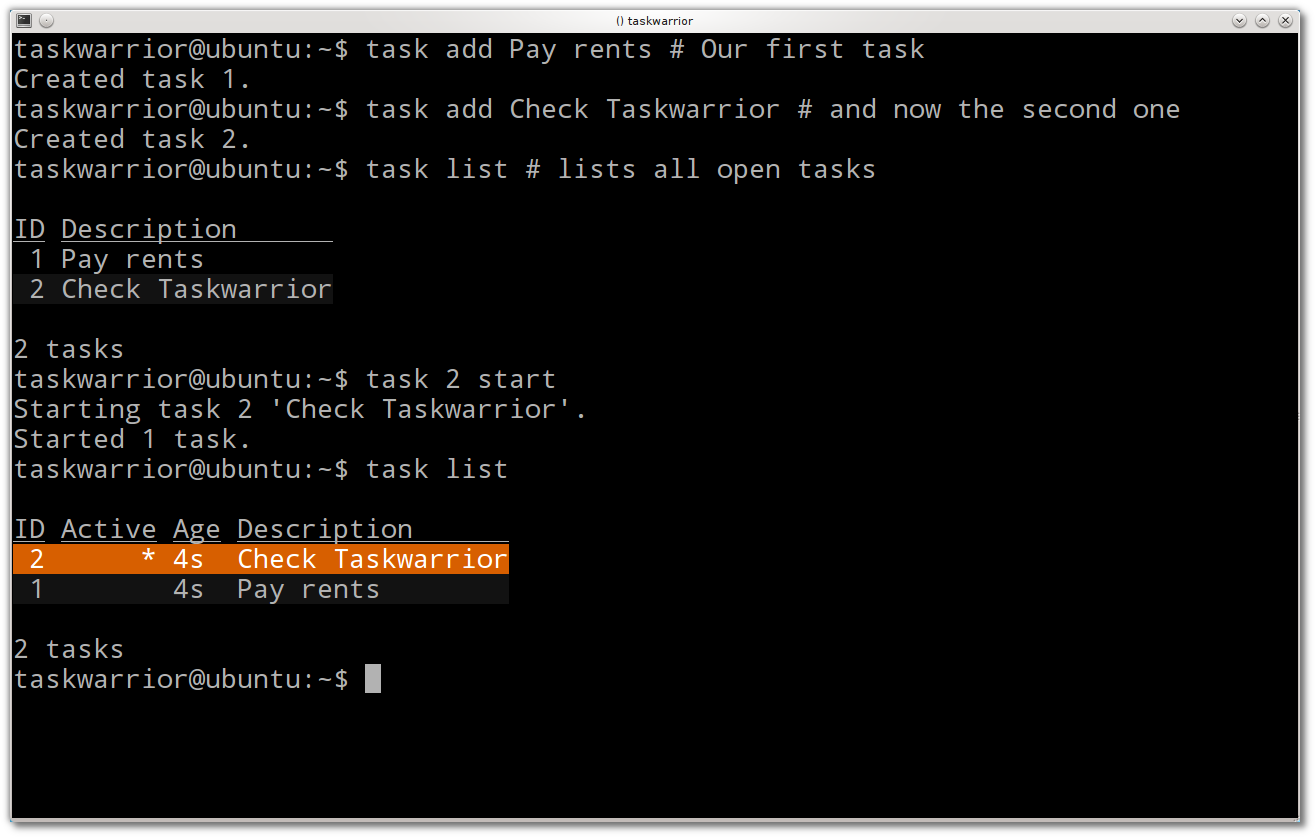
\includegraphics[width=11.8cm,height=7.5cm]{simple-example1.png}
\end{center}
%\begin{lstlisting}
%task add Pay rents # Our first task
%task add Check Taskwarrior # and now the second one
%task list # lists all open tasks
%task 2 start
%task list
%\end{lstlisting}
\end{frame}

\begin{frame}[fragile]\frametitle{A simple example, part 2}
\begin{center} % 1316x838
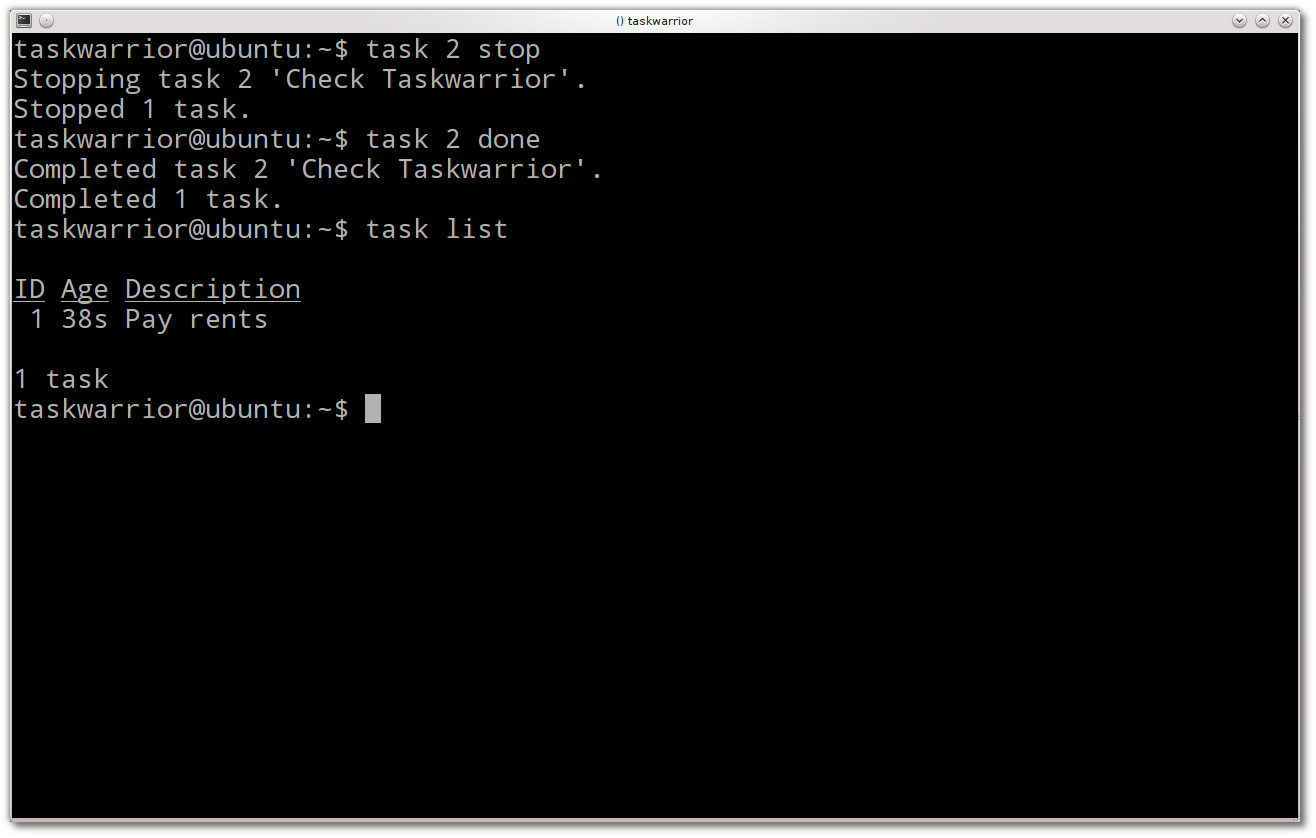
\includegraphics[width=11.8cm,height=7.5cm]{simple-example2.png}
\end{center}
%\begin{lstlisting}
%task 2 stop
%task 2 done
%task list
%\end{lstlisting}
\end{frame}

\begin{frame}\frametitle{Commands so far}
\begin{itemize}
\item \textbf{task add} \\
Adds a new task to the task list. \pause
\item \textbf{task list} \\
Provides a standard listing of tasks. \pause
\item \textbf{task start} \\
Marks the specified tasks as started. \pause
\item \textbf{task stop} \\
Removes the start time from the specified task. \pause
\item \textbf{task done} \\
Marks the specified task as done.
\end{itemize}
\end{frame}

%%%%%%%%%%%%%%%%%%%%%%%%%%%
\section{General}
%%%%%%%%%%%%%%%%%%%%%%%%%%%

\begin{frame}\frametitle{Nearly all commands work on a bunch of tasks}
\textbf{There is a lot more to explore.}

Even the commands from the last section are more mighty than they seem. \pause

\begin{itemize}
\item \textbf{task add {\tt<}mods{\tt>}}
\item \textbf{task {\tt<}filter{\tt>} list}
\item \textbf{task {\tt<}filter{\tt>} start {\tt<}mods{\tt>}}
\item \textbf{task {\tt<}filter{\tt>} stop {\tt<}mods{\tt>}}
\item \textbf{task {\tt<}filter{\tt>} done {\tt<}mods{\tt>}}
\end{itemize} \pause

To get an overview, take a look at the \href{http://taskwarrior.org/download/task-2.3.0.ref.pdf}{cheat sheet} (pdf, 145kB).
\end{frame}

\begin{frame}\frametitle{task {\tt<}filter{\tt>} command {\tt<}mods{\tt>}}
\begin{itemize} 
\item Is the basic usage of all task related write commands.
\item Write commands can operate on one task or a group of tasks or even on all tasks.
\item Every command maybe abbreviated up to the minimum that is necessary to identify a single command.
\item Filters can be anything from nothing to simple IDs further to regular expressions or Boolean constructs.
\item Modifications can be either a change of description, a change of dates or anything else that changes a task.
\item In our simple example we already used the write commands \textbf{add}, \textbf{done}, \textbf{start} and \textbf{stop}.
\end{itemize}
\end{frame}

\begin{frame}[fragile]\frametitle{Scripts}
\begin{center} % 1316x838
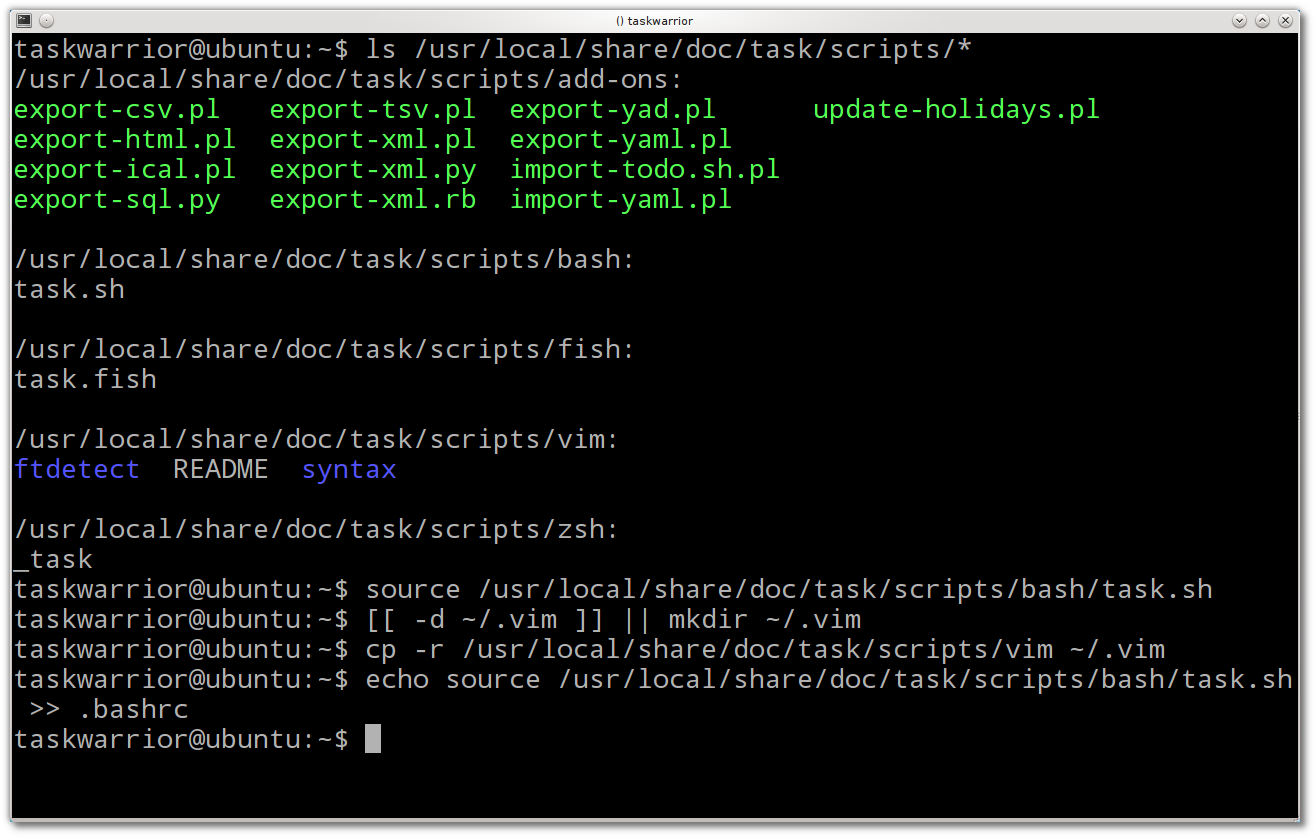
\includegraphics[width=11.8cm,height=7.5cm]{scripts.png}
\end{center}
%\begin{lstlisting}
%ls /usr/local/share/doc/task/scripts/*
%source /usr/local/share/doc/task/scripts/bash/task.sh 
%[[ -d ~/.vim ]] || mkdir ~/.vim
%cp -r /usr/local/share/doc/task/scripts/vim ~/.vim
%echo source /usr/local/share/doc/task/scripts/bash/task.sh >> .bashrc
%\end{lstlisting}
\end{frame}

\begin{frame}\frametitle{Most important commands}

These are the most important commands, just because I use them most ;-)

\begin{itemize}
\item \textbf{task {\tt<}filter{\tt>} modify} \\
The name says it, it modifies tasks according to the filter used. \pause
\item \textbf{task {\tt<}filter{\tt>} edit} \\
This starts your favourite editor with the tasks you want to change. \\
(Remember the syntax highlighting for vim?) \pause
\item \textbf{task undo} \\
Reverts the most recent change to a task. \pause
\item \textbf{task help} \\
Gives an overview of implemented commands and custom reports. \pause
\item \textbf{man task (taskrc, task-tutorial, task-color, task-faq, task-synch)} \\
Show the (almighty) man-page(s). Unlike the man-pages of many other 
programs they are extremely helpful and full of information and examples. 
Try them!
\end{itemize}
\end{frame}

%%%%%%%%%%%%%%%%%%%%%%%%%%%
\section{Working with dates}
%%%%%%%%%%%%%%%%%%%%%%%%%%%

\begin{frame}[fragile]\frametitle{Dateformats -- from 'man taskrc'}
\begin{lstlisting}
m  minimal-digit month,   for example 1 or 12
d  minimal-digit day,     for example 1 or 30
y  two-digit year,        for example 09
D  two-digit day,         for example 01 or 30
M  two-digit month,       for example 01 or 12
Y  four-digit year,       for example 2009
a  short name of weekday, for example Mon or Wed
A  long name of weekday,  for example Monday or Wednesday
b  short name of month,   for example Jan or Aug
B  long name of month,    for example January or August
V  weeknumber,            for example 03 or 37
H  two-digit hour,        for example 03 or 11
N  two-digit minutes,     for example 05 or 42
S  two-digit seconds,     for example 07 or 47

The  string may also contain other characters to act as spacers,
or formatting.  Examples for other values of dateformat:

d/m/Y  would use for input and output 24/7/2009
yMD    would use for input and output 090724
M-D-Y  would use for input and output 07-24-2009

Examples for other values of dateformat.report:

a D b Y (V)  would do an output as "Fri 24 Jul 2009 (30)"
A, B D, Y    would do an  output  as  "Friday,  July  24, 2009"
vV a Y-M-D   would do an output as "v30 Fri 2009-07-24"
yMD.HN       would do an output as "110124.2342"
m/d/Y H:N    would do an output as "1/24/2011 10:42"
a  D  b  Y  H:N:S would do and output as "Mon 24 Jan 2011 11:19:42"
\end{lstlisting}
\end{frame}

\begin{frame}[fragile]\frametitle{Set dateformat}
\begin{center} % 1316x838
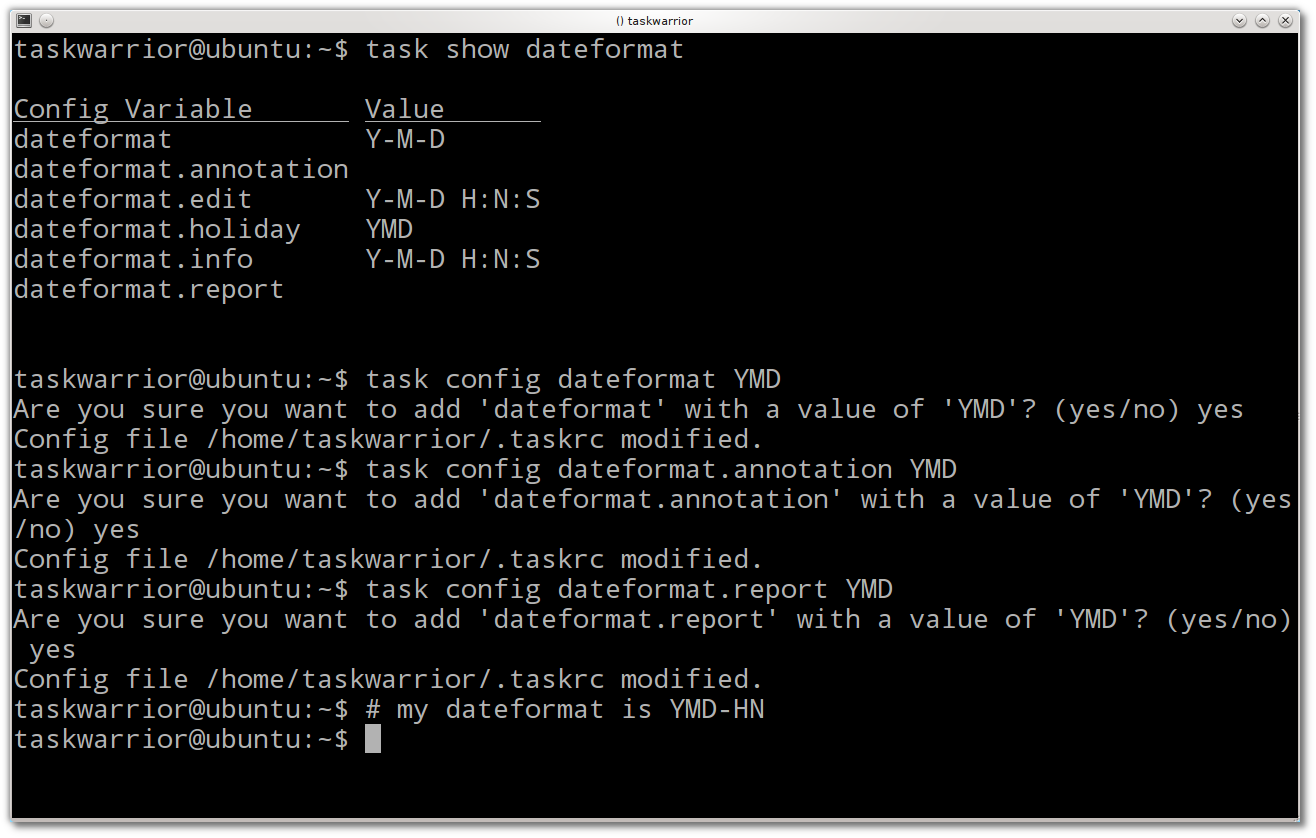
\includegraphics[width=11.8cm,height=7.5cm]{dateformat.png}
\end{center}
%\begin{lstlisting}
%task show dateformat
%task config dateformat YMD
%task config dateformat.annotation YMD
%task config dateformat.report YMD
%# my dateformat is YMD-HN
%\end{lstlisting}
\end{frame}

\begin{frame}[fragile]\frametitle{Dateformat in configuration}
\begin{center} % 1316x838
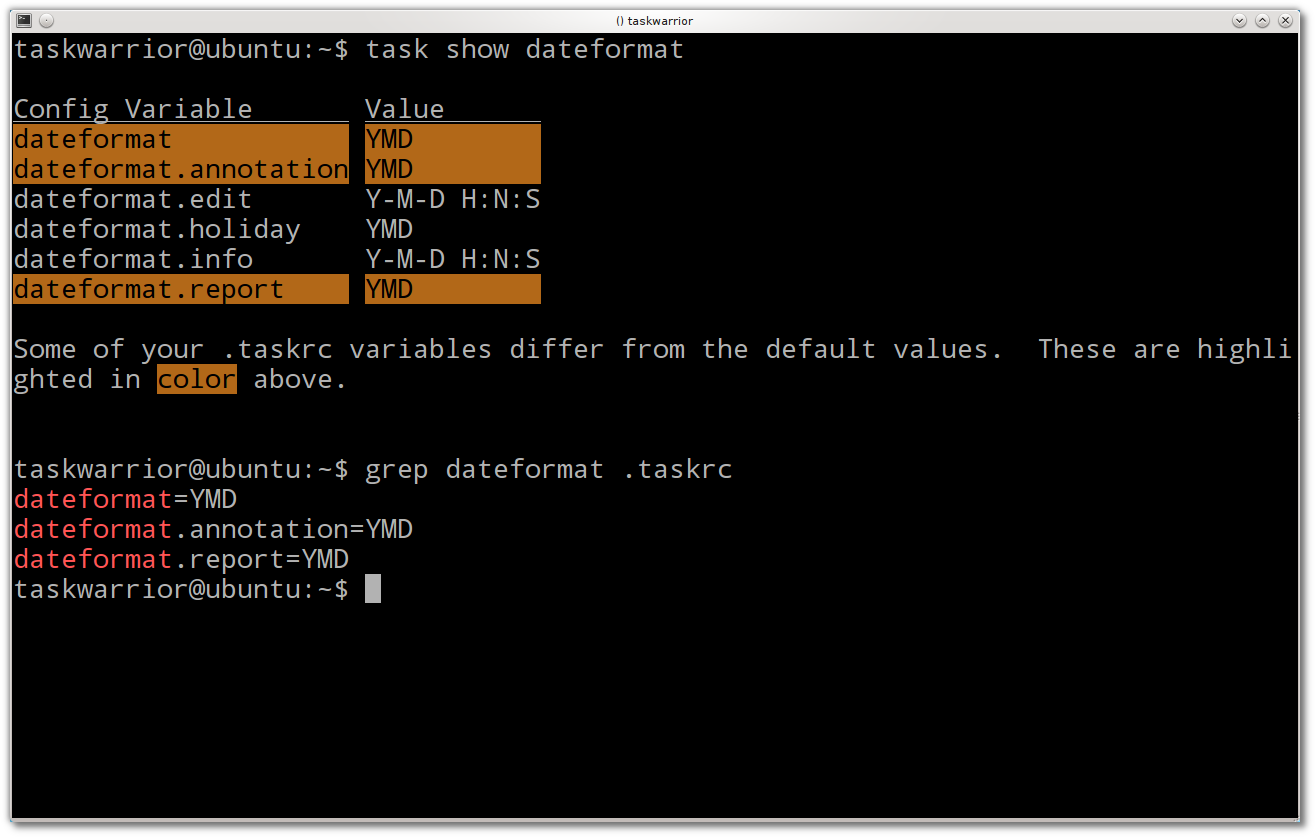
\includegraphics[width=11.8cm,height=7.5cm]{dateformat-config.png}
\end{center}
%\begin{lstlisting}
%task show dateformat
%task config dateformat YMD
%task config dateformat.annotation YMD
%task config dateformat.report YMD
%# my dateformat is YMD-HN
%\end{lstlisting}
\end{frame}

\begin{frame}[fragile]\frametitle{Set weekstart}
\begin{center} % 1316x838
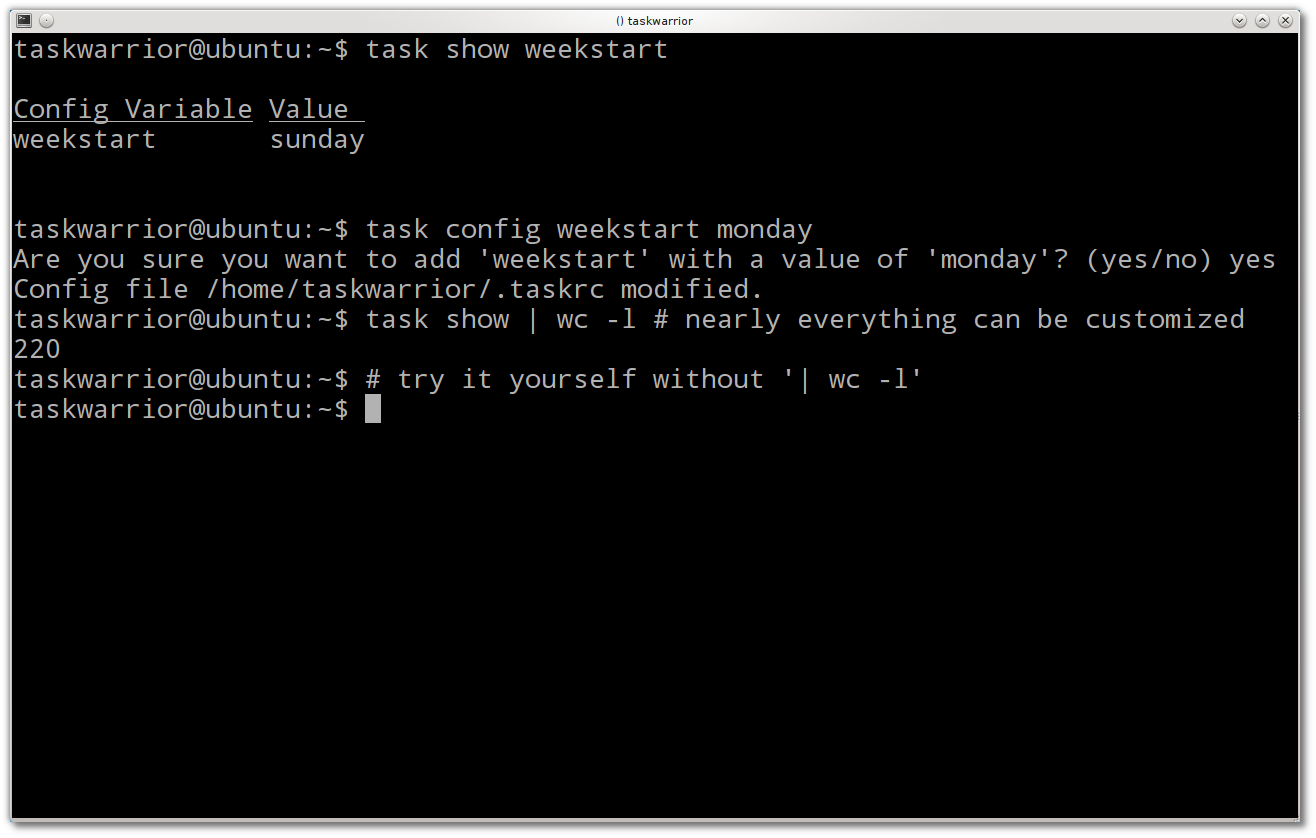
\includegraphics[width=11.8cm,height=7.5cm]{weekstart.png}
\end{center}
%\begin{lstlisting}
%$ task show weekstart
%$ task config weekstart Monday
%$ task show | wc -l # nearly everything can be customized
%220
%$ # try it yourself without '| wc -l'
%\end{lstlisting}
\end{frame}

\begin{frame}\frametitle{Special dates (1)}
\begin{itemize}
\item \textbf{Relative wording} \\
task ... due:today \\
task ... due:yesterday \\
task ... due:tomorrow \\
\item \textbf{Day number with ordinal} \\
task ... due:23rd \\
task ... due:3wks \\
task ... due:1day \\
task ... due:9hrs \\
\item \textbf{At some point or later} \\
task ... wait:later
task ... wait:someday
This sets the wait date to 1/18/2038.
\end{itemize}
\end{frame}

\begin{frame}\frametitle{Special dates (2)}
\begin{itemize}
\item \textbf{Start / end of (work) week, calendar week (according to settings of weekstart), month, quarter and year} \\
task ... due:sow \\
task ... due:eow \\
task ... due:soww \\
task ... due:eoww \\
task ... due:socw \\
task ... due:eocw \\
task ... due:som \\
task ... due:eom \\
task ... due:soq \\
task ... due:eoq \\
task ... due:soy \\
task ... due:eoy \\
\item \textbf{Next occurring weekday} \\
task ... due:fri
\end{itemize}
\end{frame}

\begin{frame}[fragile]\frametitle{Due and wait}
\begin{center} % 1316x838
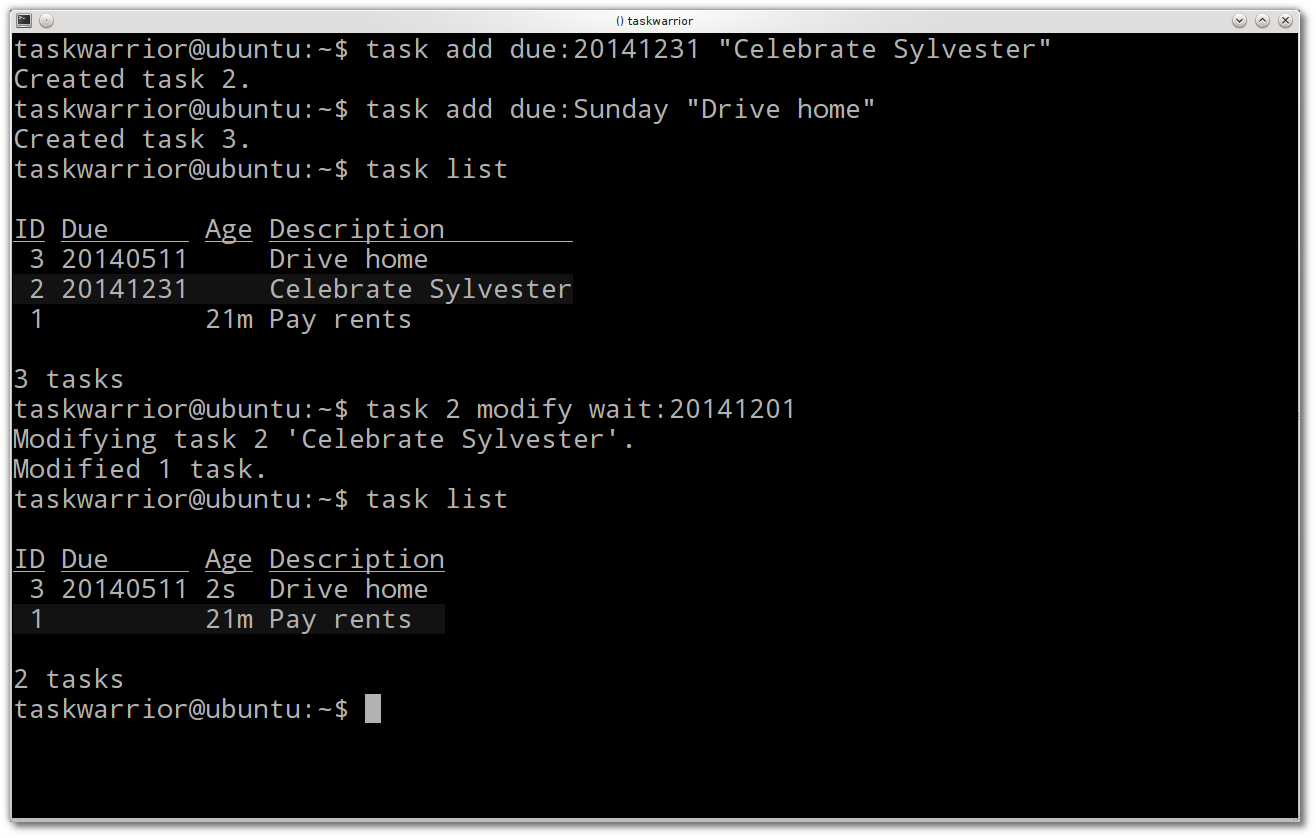
\includegraphics[width=11.8cm,height=7.5cm]{due-and-wait.png}
\end{center}
%\begin{lstlisting}
%task add due:20141231 "Celebrate Sylvester"
%task add due:Sunday "Drive home"
%task list
%task 2 modify wait:20141201
%task list
%\end{lstlisting}
\end{frame}

\begin{frame}[fragile]\frametitle{Recurrence}
\begin{center} % 1316x838
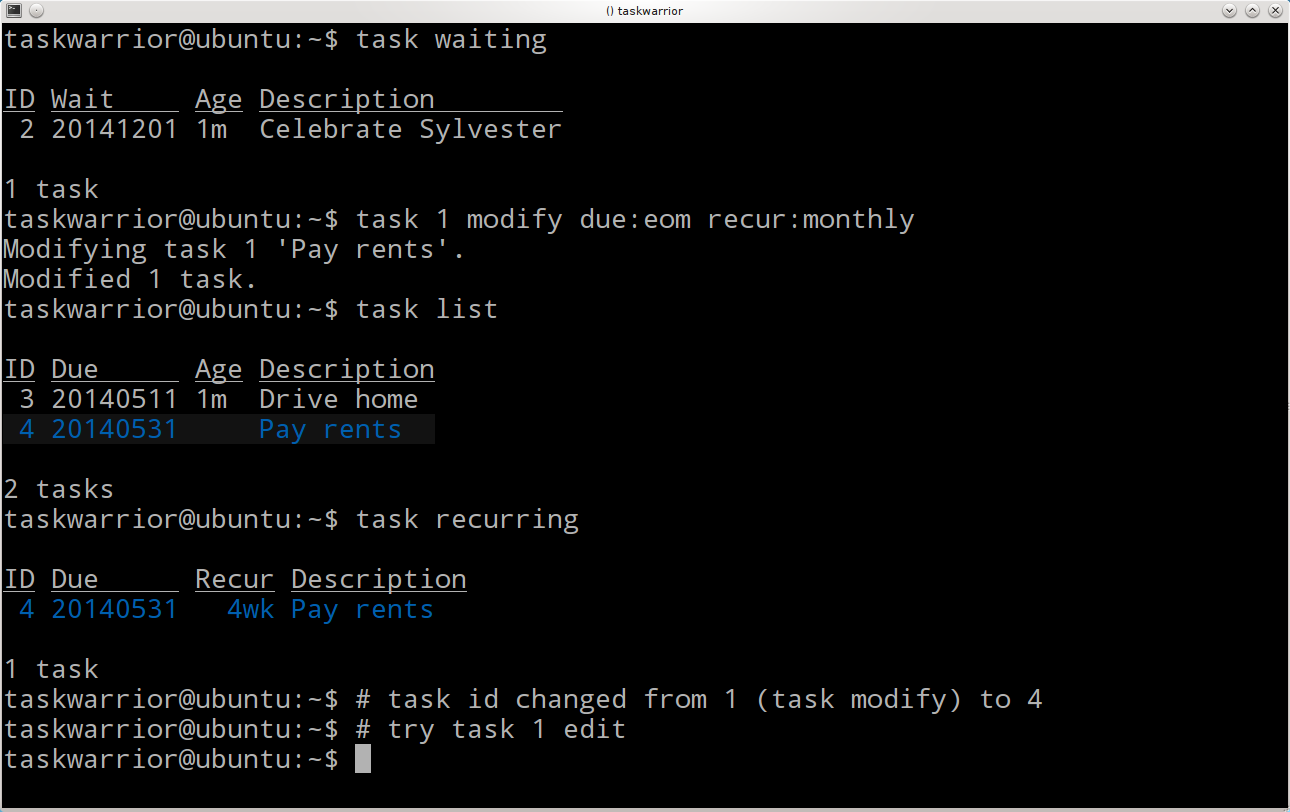
\includegraphics[width=11.8cm,height=7.5cm]{recurrence.png}
\end{center}
%\begin{lstlisting}
%task waiting
%task 1 modify due:eom recur:monthly
%task list
%task recurring
%# task id changed from 1 (task modify) to 4
%# try task 1 edit
%\end{lstlisting}
\end{frame}

\begin{frame}\frametitle{Recurrence modifiers (1)}
\begin{itemize}
\item \textbf{hourly} \\
Every hour.
\item \textbf{daily, day, 1da, 2da, ...} \\
Every day or a number of days.
\item \textbf{weekdays} \\
Mondays, Tuesdays, Wednesdays, Thursdays, Fridays and skipping  weekend days.
\item \textbf{weekly, 1wk, 2wks, ...} \\
Every week or a number of weeks.
\item \textbf{biweekly, fortnight} \\
Every two weeks.
\item \textbf{monthly} \\
Every month.
\item \textbf{quarterly, 1qtr, 2qtrs, ...} \\
Every three months, a quarter, or a number of quarters.
\end{itemize}
\end{frame}

\begin{frame}\frametitle{Recurrence modifiers (2)}
\begin{itemize}
\item \textbf{semiannual} \\
Every six months.
\item \textbf{annual, yearly, 1yr, 2yrs, ...} \\
Every year or a number of years.
\item \textbf{biannual, biyearly, 2yr} \\
Every two years.
\end{itemize}
\end{frame}

\begin{frame}[fragile]\frametitle{Until and entry}
\begin{center} % 1316x838
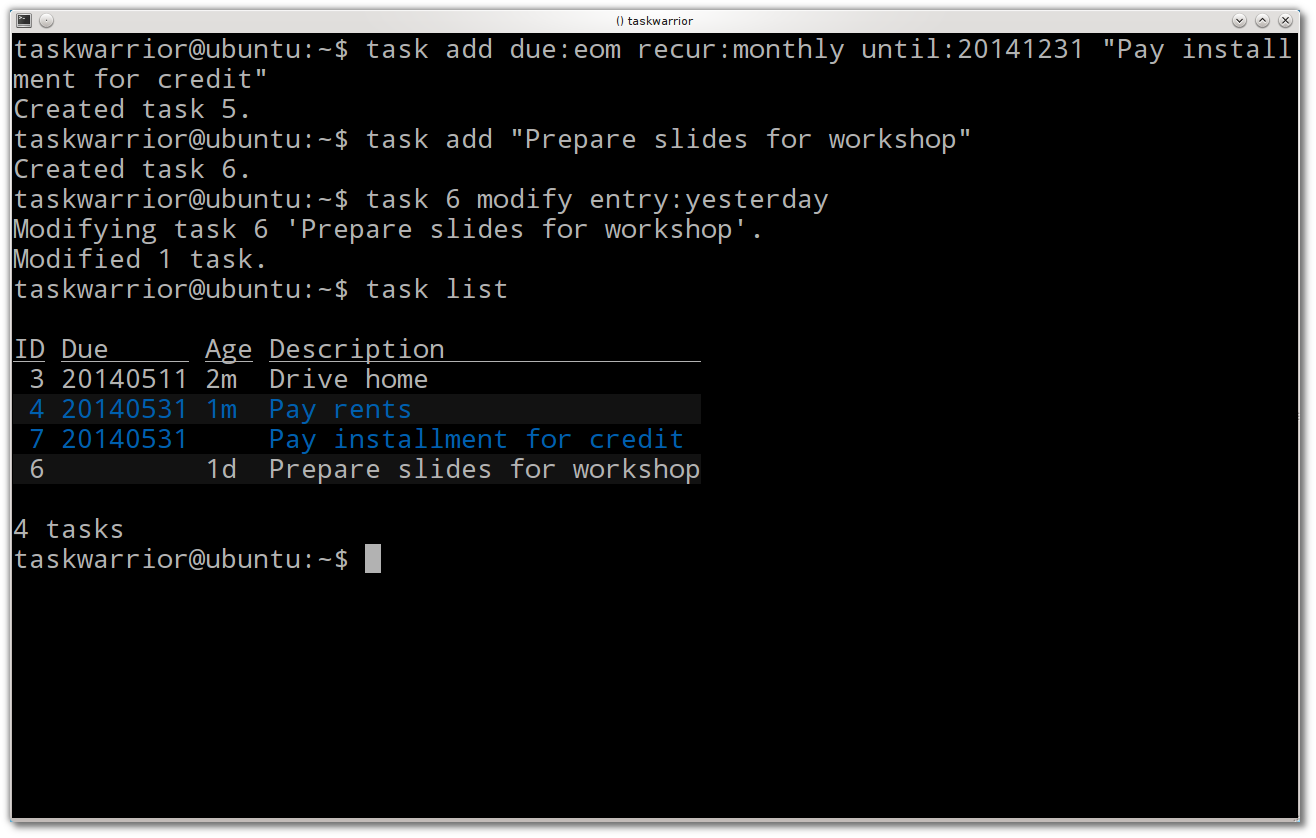
\includegraphics[width=11.8cm,height=7.5cm]{until-and-entry.png}
\end{center}
%\begin{lstlisting}
%task add due:eom recur:monthly until:20141231 "Pay installment for credit"
%ask add "Prepare slides for workshop"
%ask 6 modify entry:yesterday
%task list
%\end{lstlisting}
\end{frame}

\begin{frame}[fragile]\frametitle{Starting and stopping}
\begin{center} % 1316x838
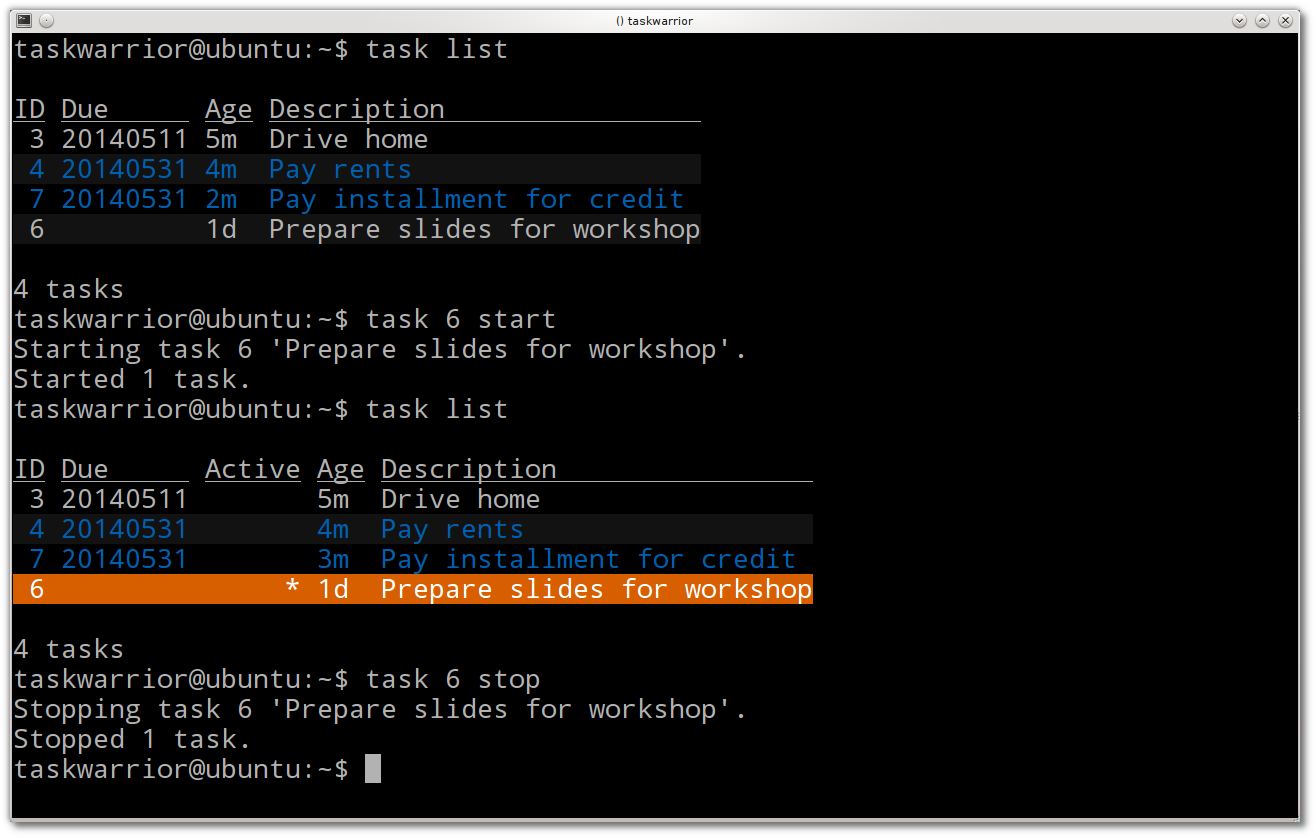
\includegraphics[width=11.8cm,height=7.5cm]{starting-and-stopping.png}
\end{center}
%\begin{lstlisting}
%task list
%task 10 start
%task list
%task 10 stop
%\end{lstlisting}
\end{frame}

\begin{frame}\frametitle{Holiday}
\begin{alertblock}{Attention!}
Holiday has nothing in common with the German words "'Ferien"' or "'Urlaub"' (this would be vacation). (Public) Holiday means "'Feiertag"'.
\end{alertblock}

You can add holidays by either adding them via "'task config"' on the commandline or by adding them directly to the ~/.taskrc-File or by including an external holiday definition.

On \href{http://holidata.net/}{holidata.net} you find a growing list of holiday dates, licensed CC-BY and offered by volunteers. Service was introduced by the Taskwarrior team, who is responsible for hosting and conversion to different formats.
\end{frame}

\begin{frame}[fragile]\frametitle{Add holiday}
\begin{center} % 1316x838
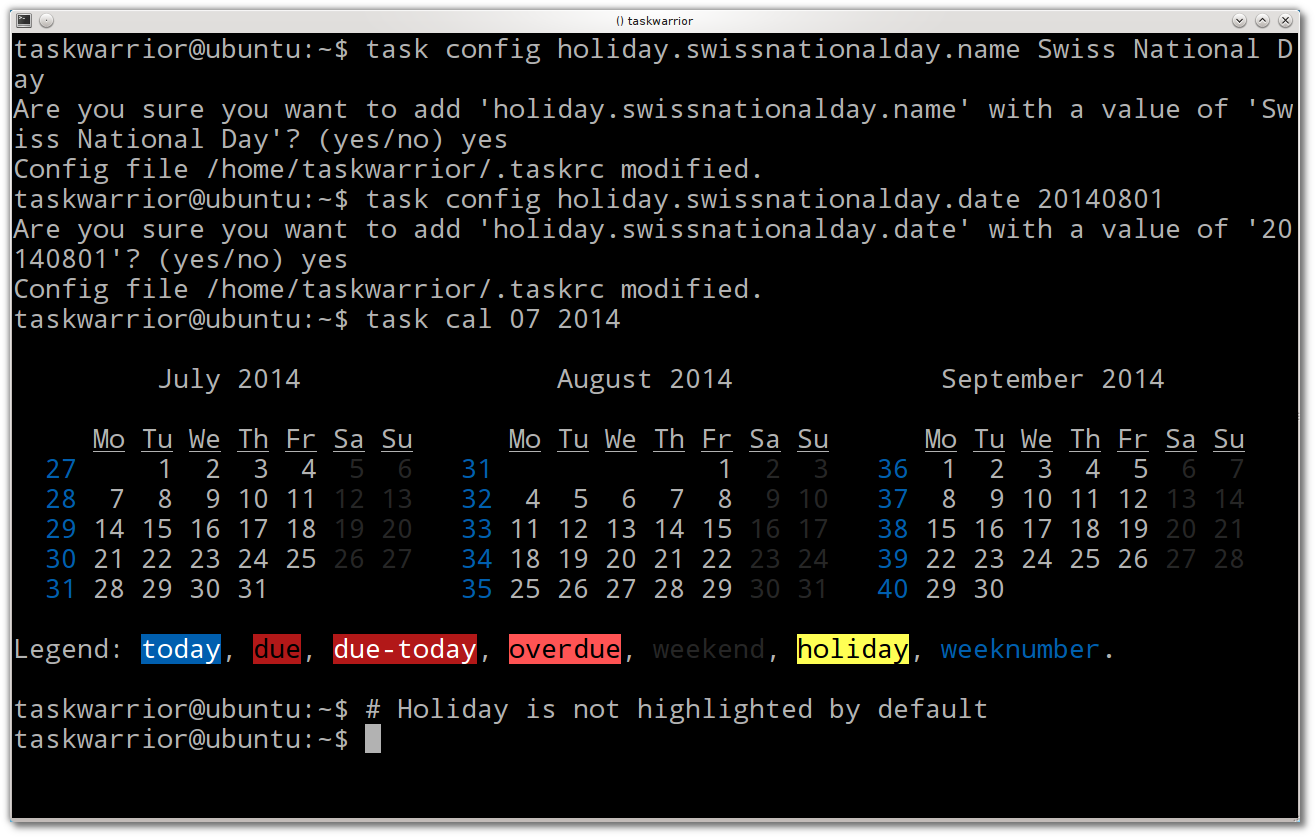
\includegraphics[width=11.8cm,height=7.5cm]{add-holiday.png}
\end{center}
%\begin{lstlisting}
%task config holiday.swissnationalday.name Swiss National Day
%task config holiday.swissnationalday.date 20140801
%task cal 07 2014
%# Holiday is not highlighted by default
%\end{lstlisting}
\end{frame}

\begin{frame}[fragile]\frametitle{Calendar config with holiday}
\begin{center} % 1316x838
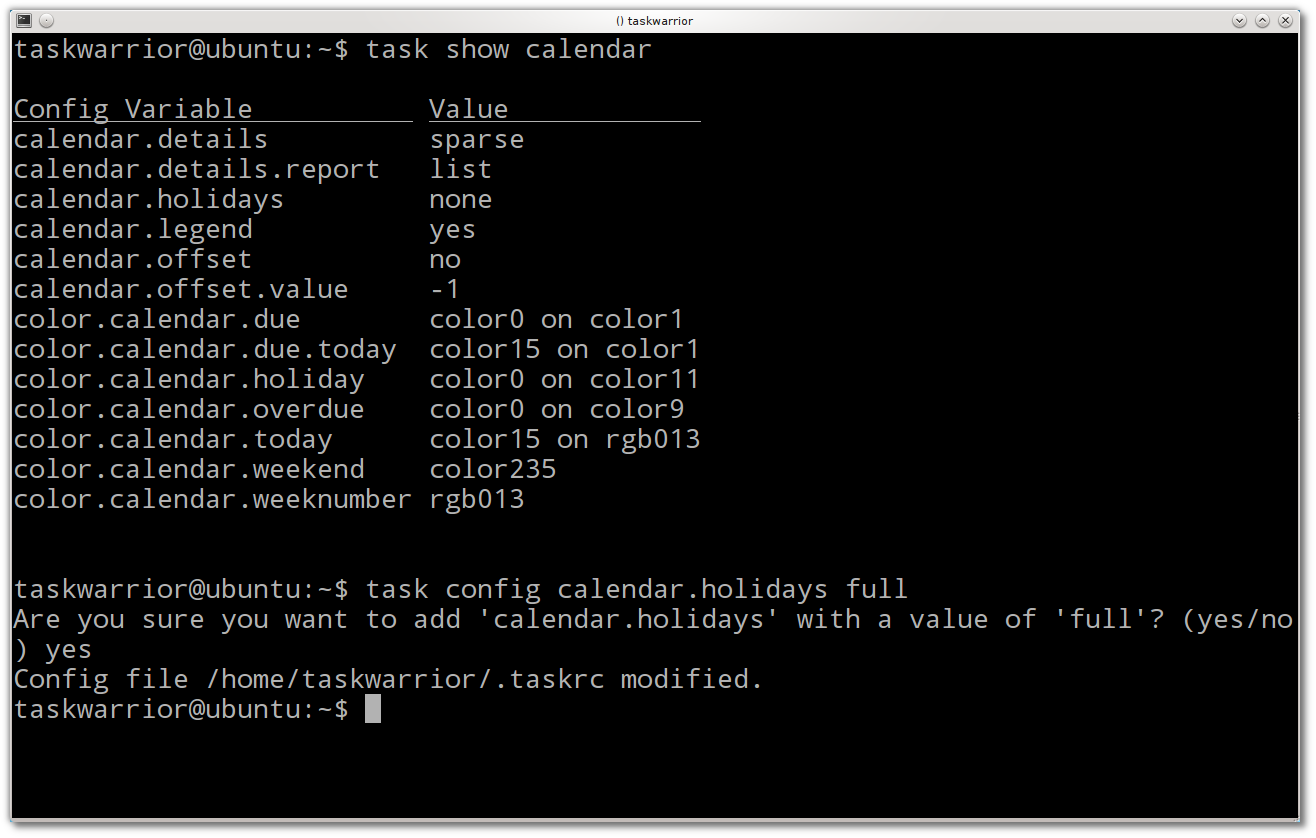
\includegraphics[width=11.8cm,height=7.5cm]{calendar-config-with-holiday.png}
\end{center}
%\begin{lstlisting}
%task show calendar
%task config calendar.holidays full
%\end{lstlisting}
\end{frame}

\begin{frame}[fragile]\frametitle{Calendar with holiday}
\begin{center} % 1316x838
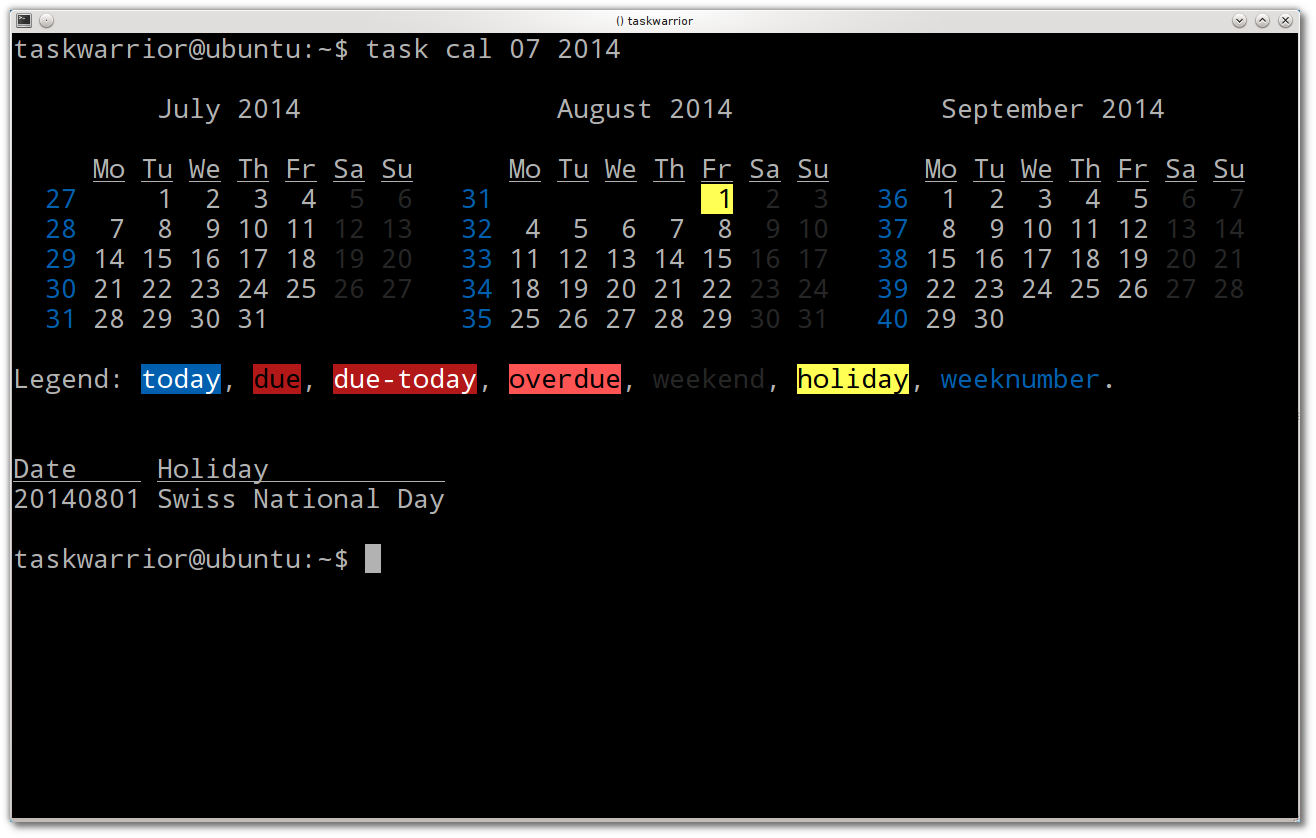
\includegraphics[width=11.8cm,height=7.5cm]{calendar-with-holiday.png}
\end{center}
%\begin{lstlisting}
%task cal 07 2014
%\end{lstlisting}
\end{frame}

\begin{frame}[fragile]\frametitle{Calendar with due tasks}
\begin{center} % 1316x838
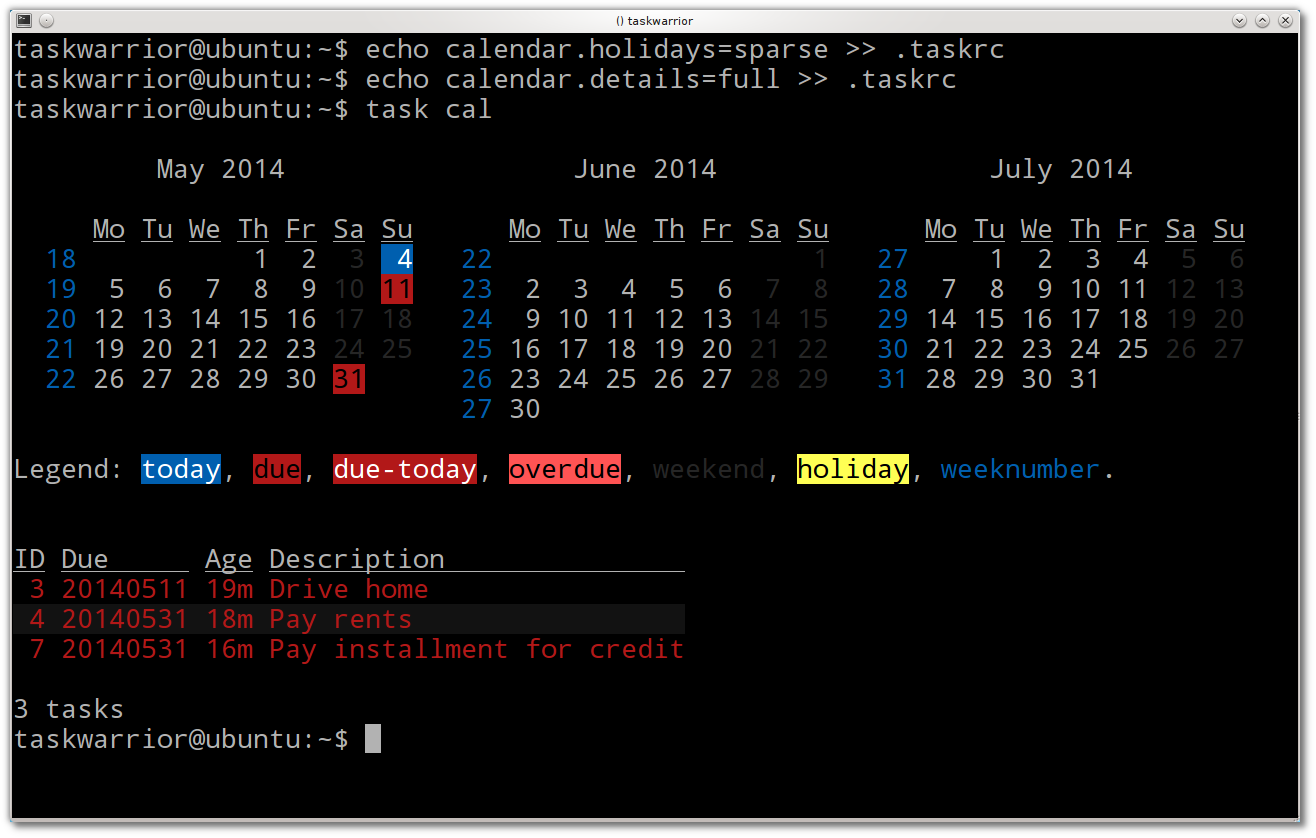
\includegraphics[width=11.8cm,height=7.5cm]{calendar-with-due-tasks.png}
\end{center}
%\begin{lstlisting}
%task config calendar.holidays sparse 
%task config calendar.details full
%task cal
%\end{lstlisting}
\end{frame}

\begin{frame}[fragile]\frametitle{Timesheet}
\begin{center} % 1316x838
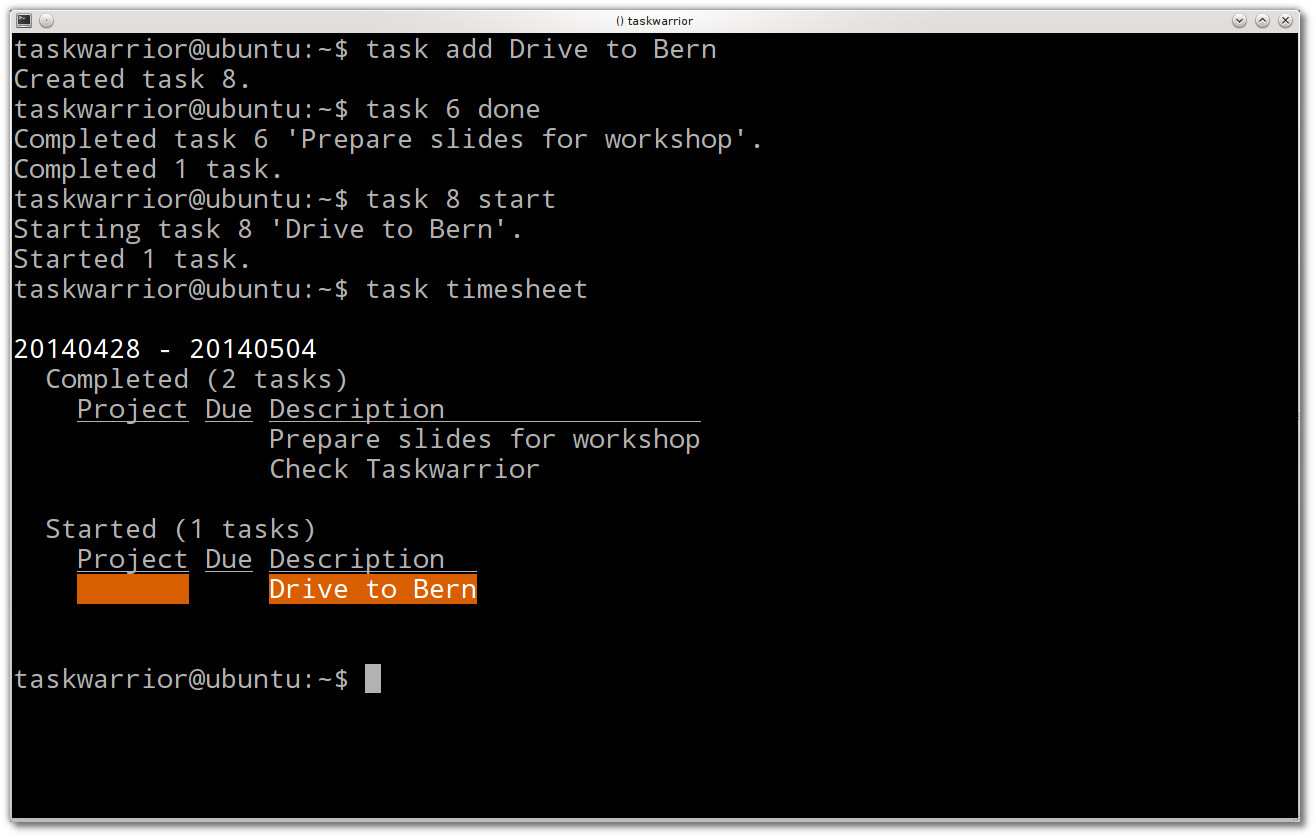
\includegraphics[width=11.8cm,height=7.5cm]{timesheet.png}
\end{center}
%\begin{lstlisting}
%task add Drive to Leipzig
%task 6 done
%task 8 start
%task timesheet
%\end{lstlisting}
\end{frame}

%%%%%%%%%%%%%%%%%%%%%%%%%%%
\section{Getting sorted}
%%%%%%%%%%%%%%%%%%%%%%%%%%%

\begin{frame}[fragile]\frametitle{Project and subproject}
\begin{center} % 1316x838
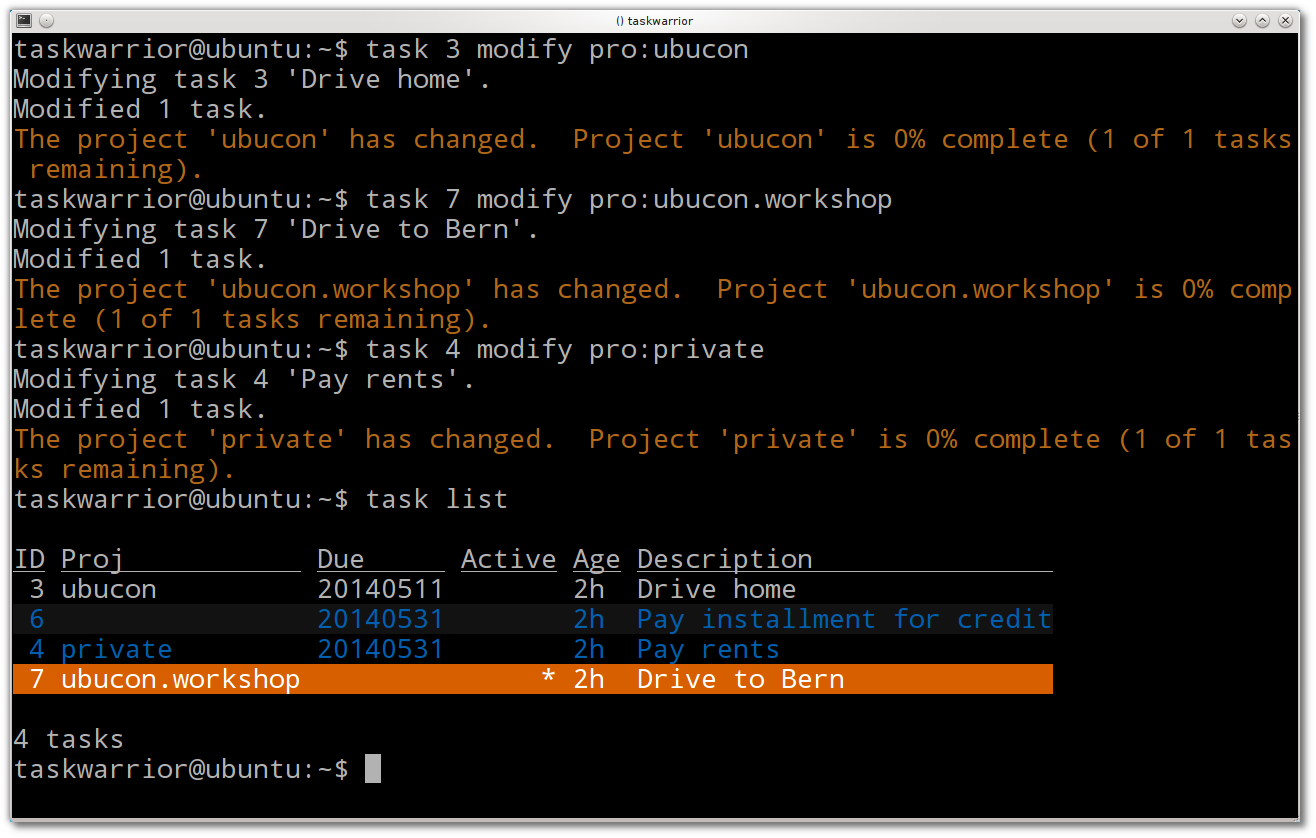
\includegraphics[width=11.8cm,height=7.5cm]{project-and-subproject.png}
\end{center}
%\begin{lstlisting}
%task 3 modify pro:ubucon
%task 7 modify pro:ubucon.workshop
%task 4 modify pro:private
%task list
%\end{lstlisting}
\end{frame}

\begin{frame}[fragile]\frametitle{Projects}
\begin{center} % 1316x838
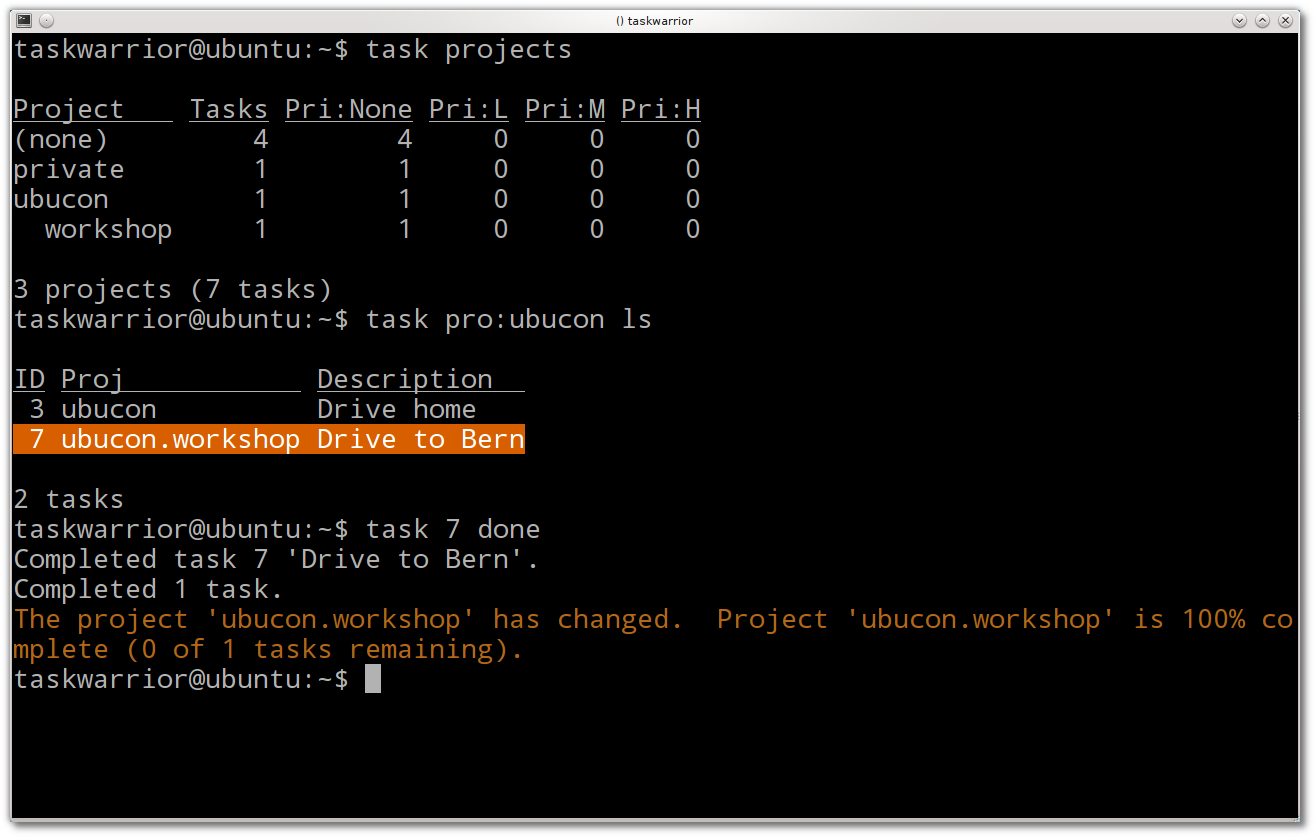
\includegraphics[width=11.8cm,height=7.5cm]{projects.png}
\end{center}
%\begin{lstlisting}
%task projects
%task pro:ubucon ls
%task 7 done
%\end{lstlisting}
\end{frame}

\begin{frame}[fragile]\frametitle{Tags}
\begin{center} % 1316x838
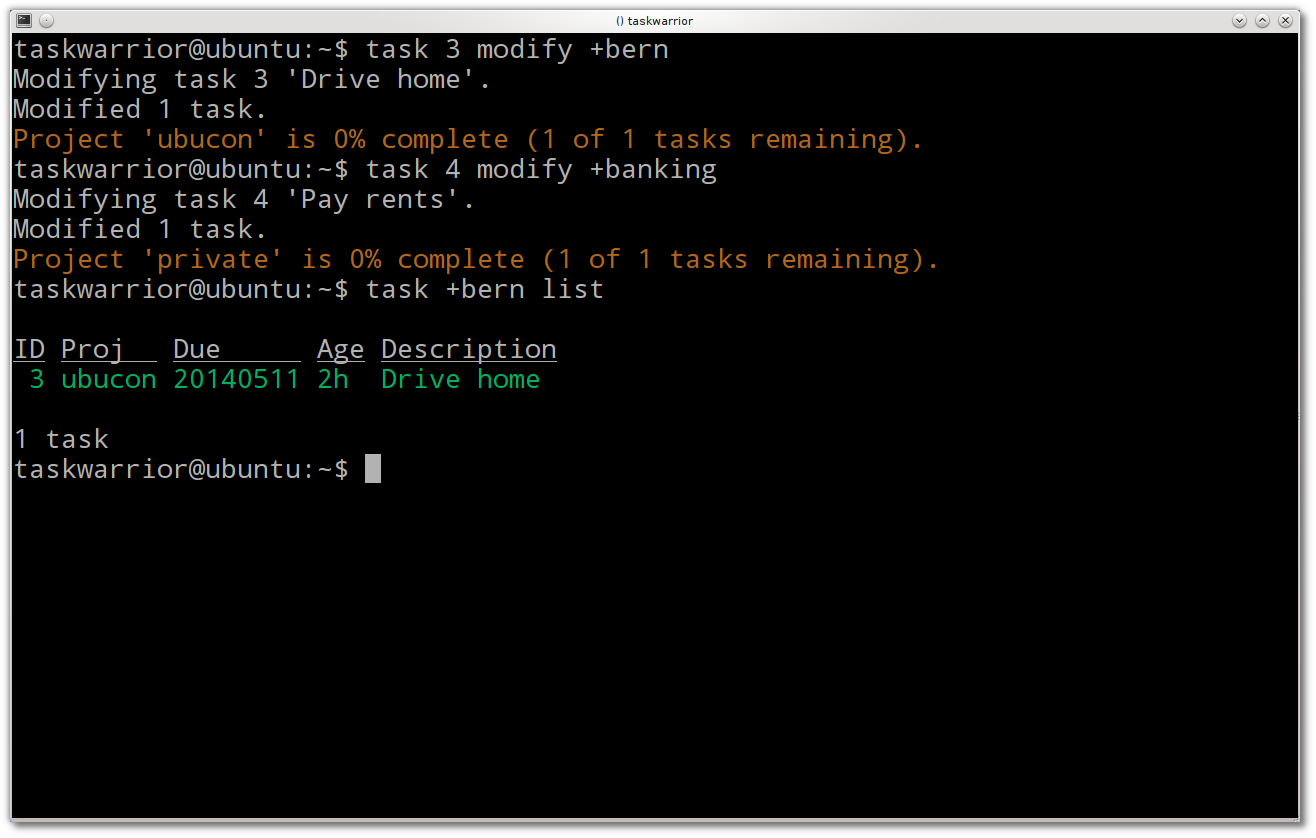
\includegraphics[width=11.8cm,height=7.5cm]{tags.png}
\end{center}
%\begin{lstlisting}
%task 3 modify +bern
%task 4 modify +banking
%task +bern list
%\end{lstlisting}
\end{frame}

\begin{frame}[fragile]\frametitle{Priorities}
\begin{center} % 1316x838
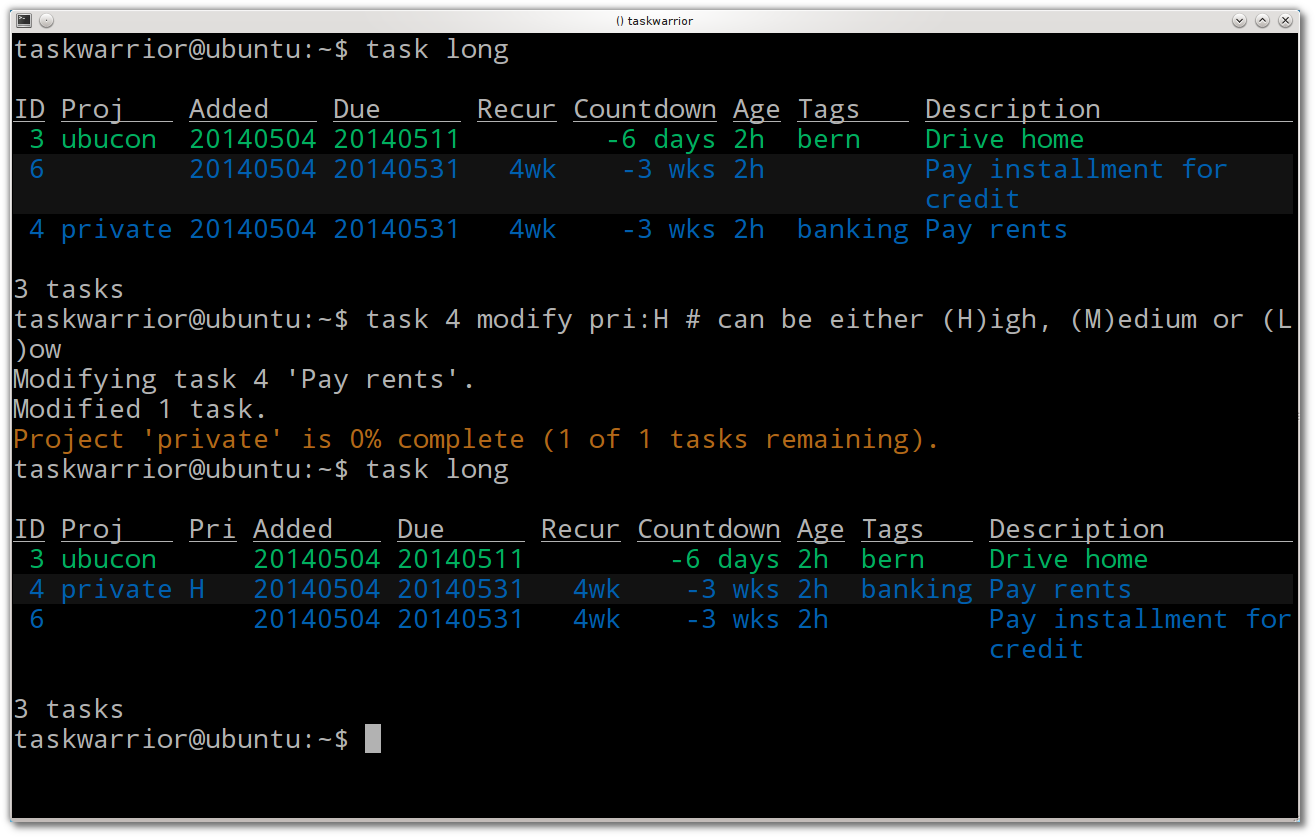
\includegraphics[width=11.8cm,height=7.5cm]{priorities.png}
\end{center}
%\begin{lstlisting}
%task long
%task 4 modify pri:H # can be either (H)igh, (M)edium or (L)ow
%task long
%\end{lstlisting}
\end{frame}

\begin{frame}[fragile]\frametitle{Annotations}
\begin{center} % 1316x838
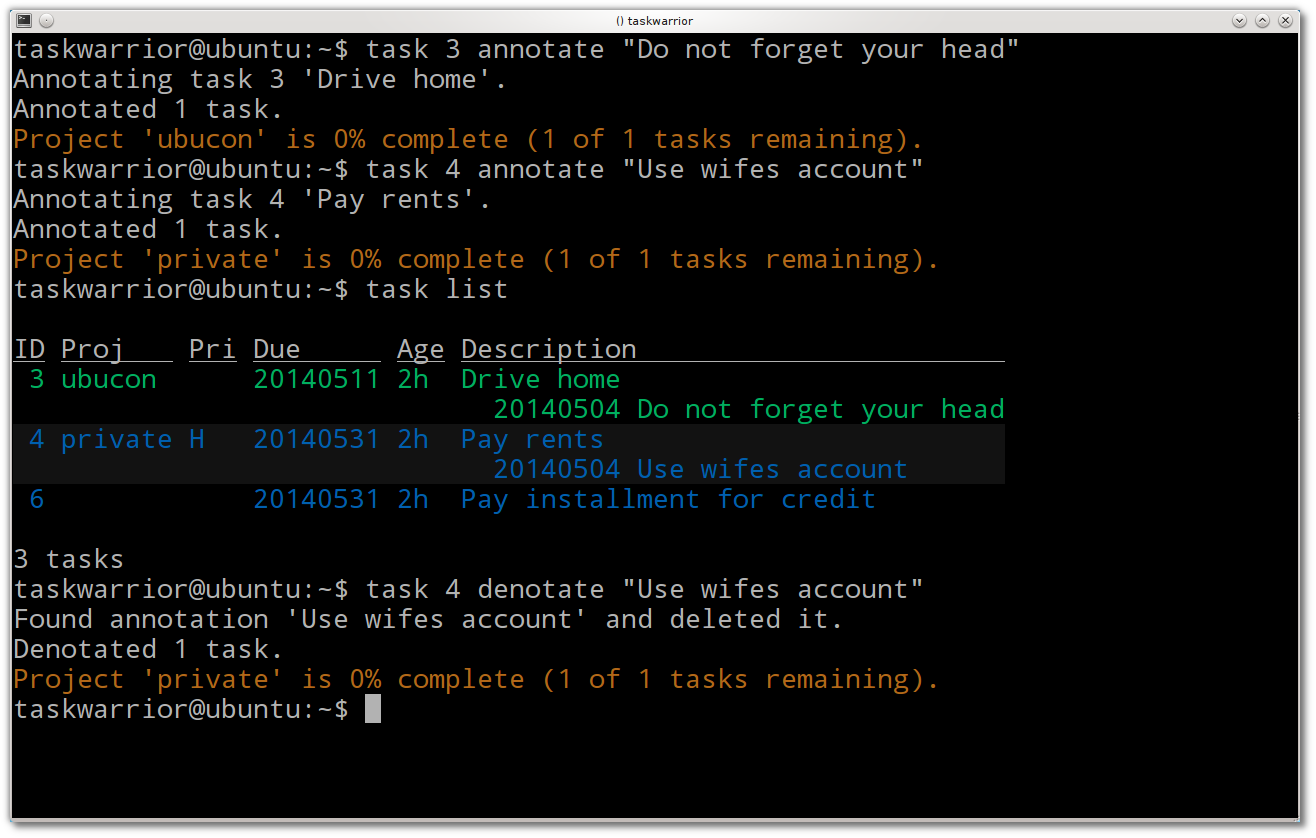
\includegraphics[width=11.8cm,height=7.5cm]{annotations.png}
\end{center}
%\begin{lstlisting}
%task 3 annotate "Do not forget your head"
%task 4 annotate "Use wifes account"
%task list
%task 4 denotate "Use wifes account"
%\end{lstlisting}
\end{frame}

%%%%%%%%%%%%%%%%%%%%%%%%%%%
\section{Dependencies}
%%%%%%%%%%%%%%%%%%%%%%%%%%%

\begin{frame}[fragile]\frametitle{Dependency, part 1}
\begin{center} % 1316x838
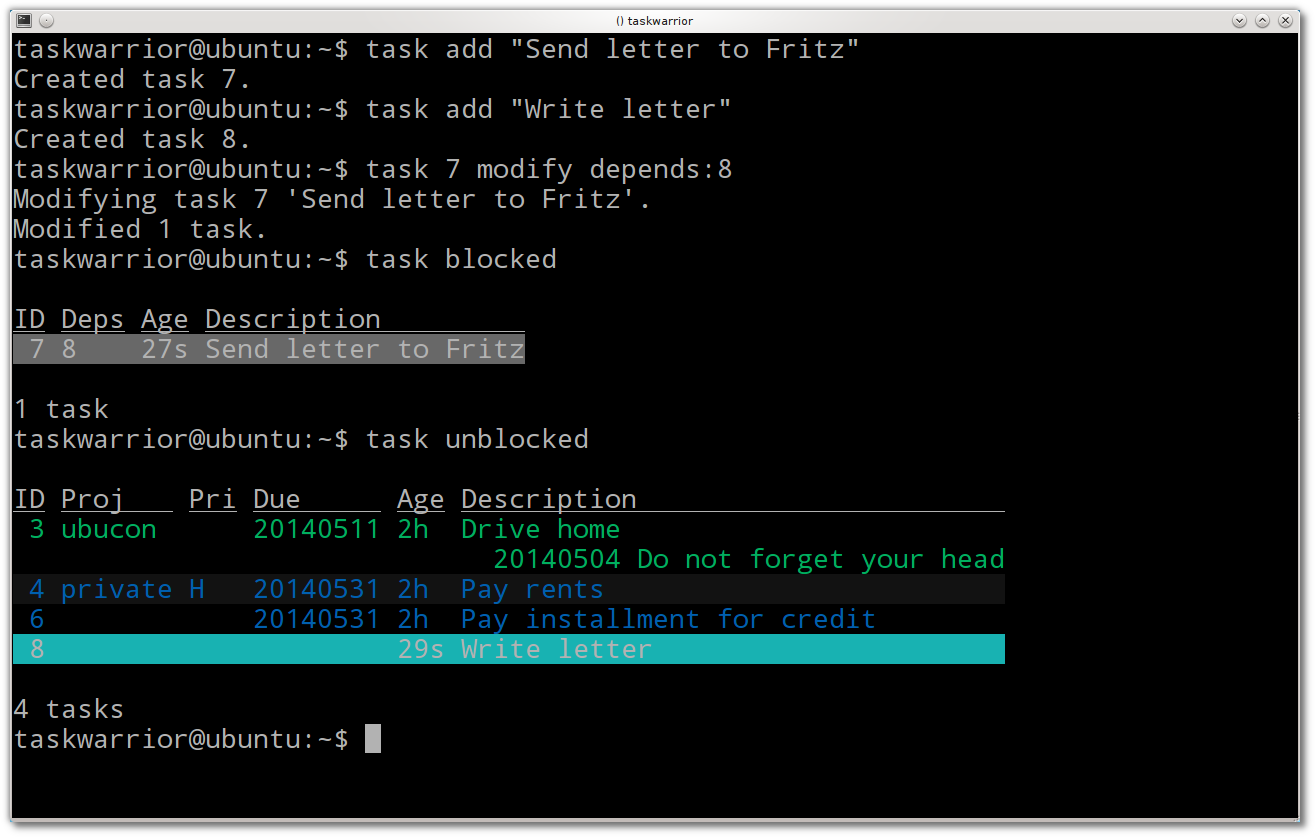
\includegraphics[width=11.8cm,height=7.5cm]{dependency1.png}
\end{center}
%\begin{lstlisting}
%task add "Send letter to Fritz"
%task add "Write letter"
%task 7 modify depends:8
%task blocked
%task unblocked
%\end{lstlisting}
\end{frame}

\begin{frame}[fragile]\frametitle{Dependency, part 2}
\begin{center} % 1316x838
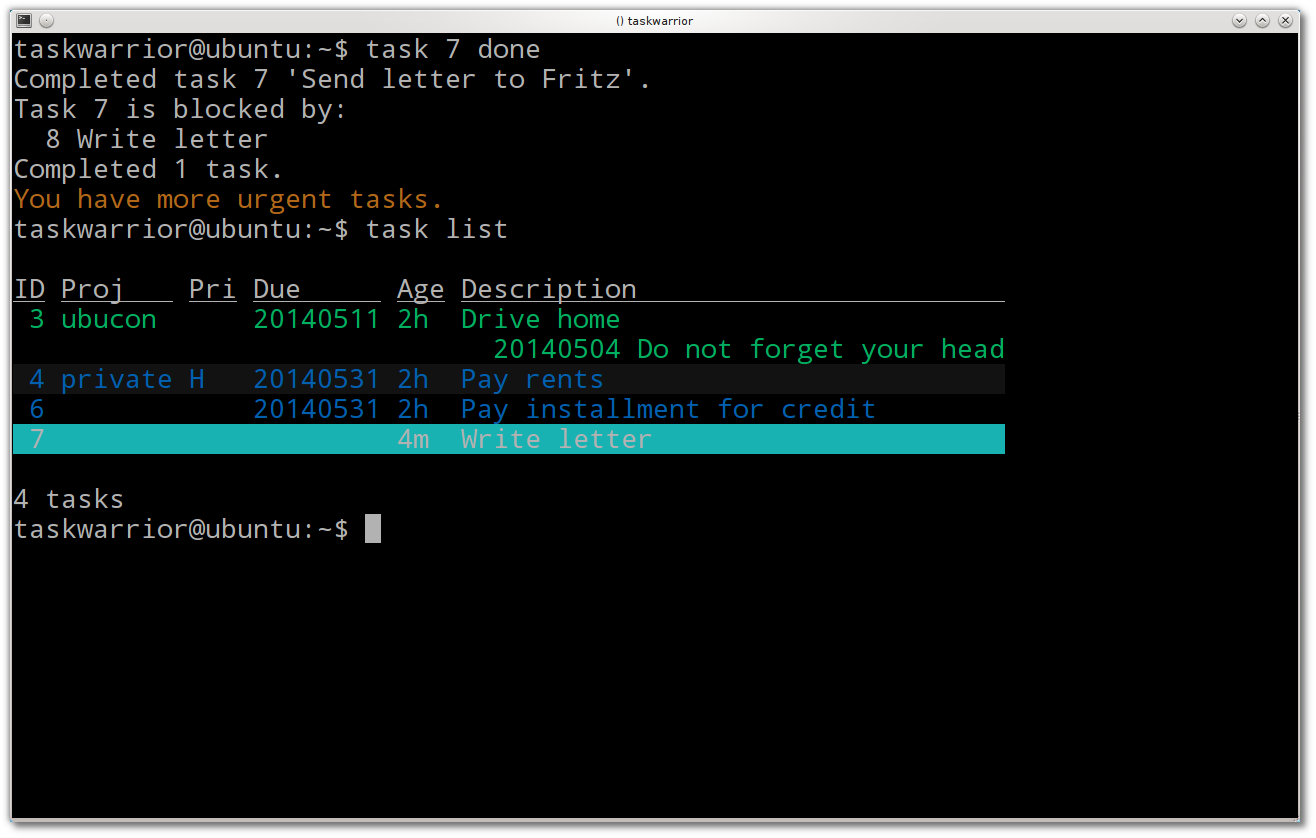
\includegraphics[width=11.8cm,height=7.5cm]{dependency2.png}
\end{center}
%\begin{lstlisting}
%task 7 done
%task list
%\end{lstlisting}
\end{frame}

\begin{frame}[fragile]\frametitle{Undo}
\begin{center} % 1316x838
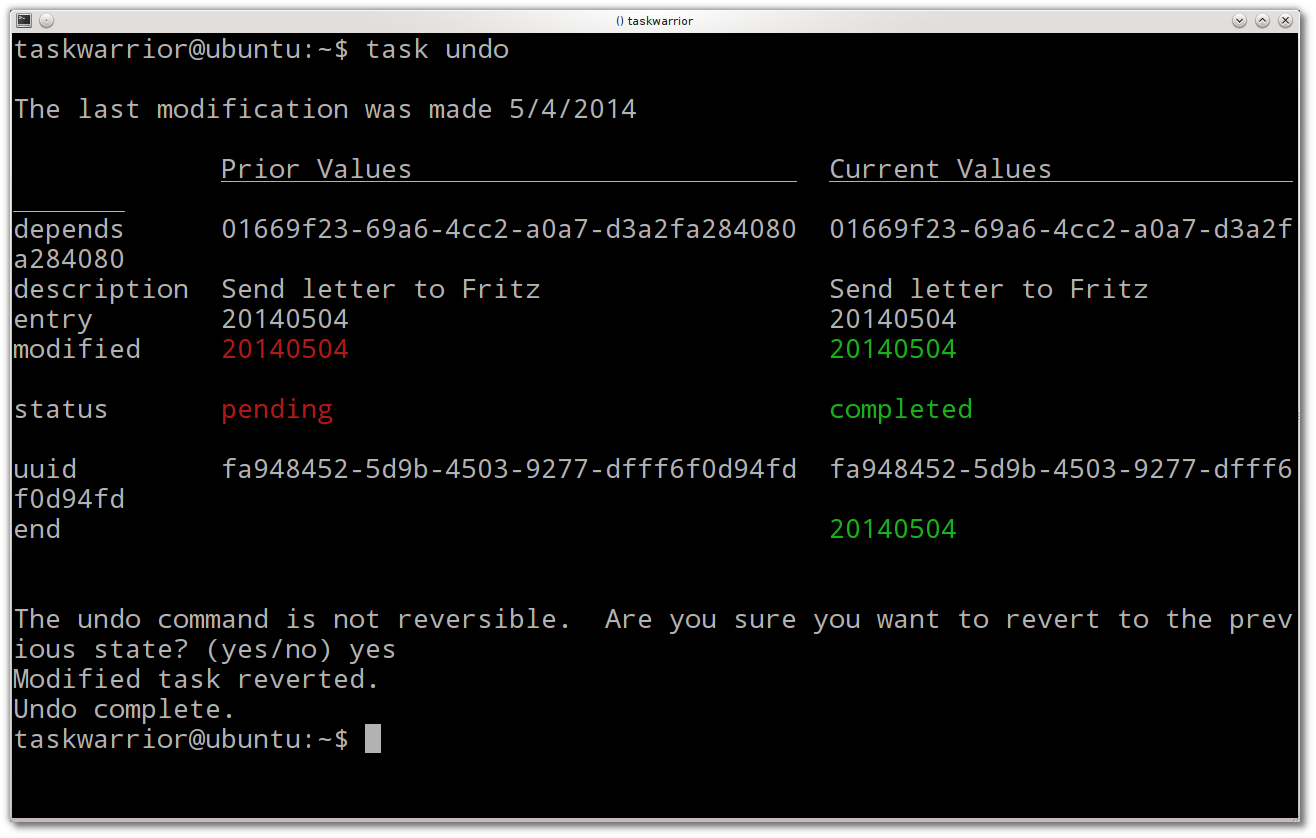
\includegraphics[width=11.8cm,height=7.5cm]{undo.png}
\end{center}
%\begin{lstlisting}
%task undo
%\end{lstlisting}
\end{frame}

\begin{frame}[fragile]\frametitle{Dependency, part 3}
\begin{center} % 1316x838
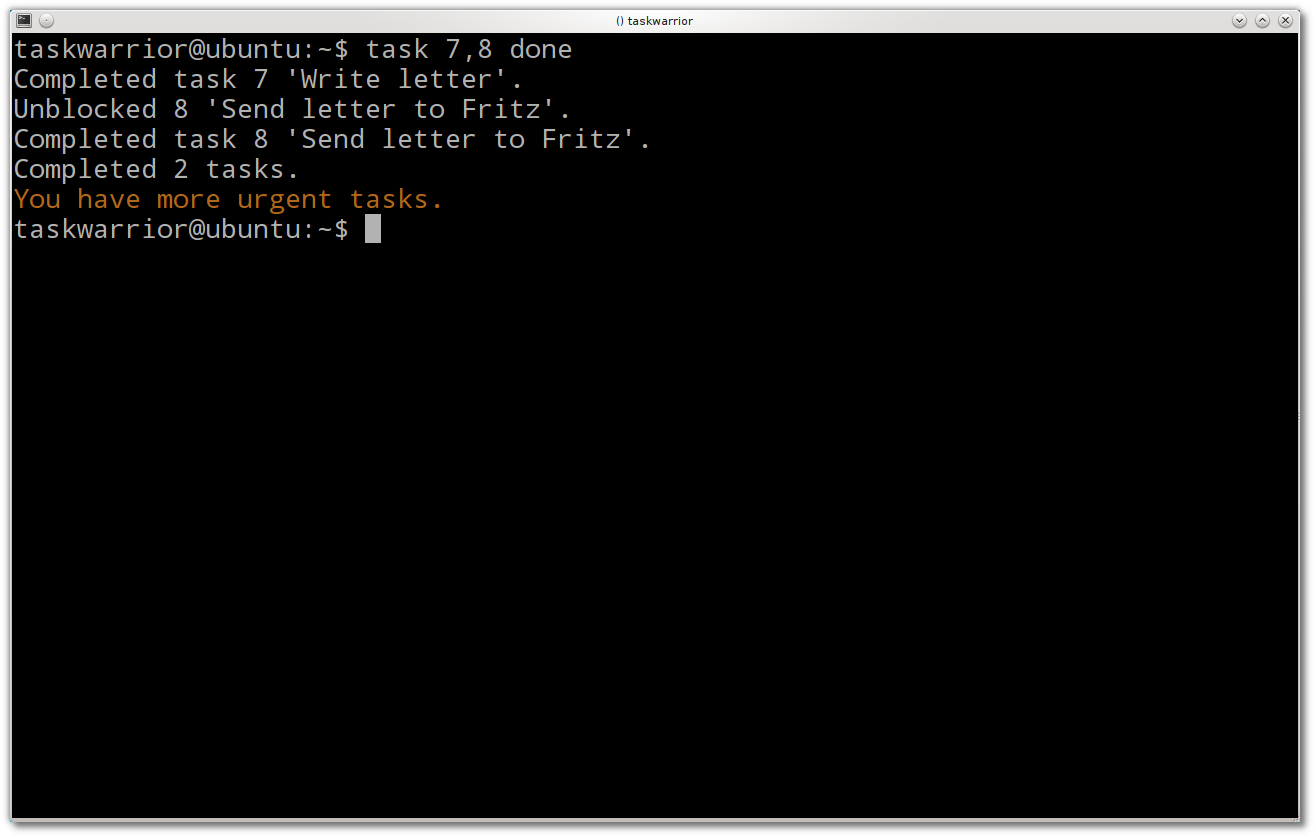
\includegraphics[width=11.8cm,height=7.5cm]{dependency3.png}
\end{center}
%\begin{lstlisting}
%task 7,8 done
%task blocked
%\end{lstlisting}
\end{frame}

%%%%%%%%%%%%%%%%%%%%%%%%%%%
\section{Reports}
%%%%%%%%%%%%%%%%%%%%%%%%%%%

\begin{frame}\frametitle{Predefined reports (from task reports), part 1}

These reports were already used.

\begin{itemize}
\item \textbf{blocked}          Lists all blocked tasks matching the specified criteria
\item \textbf{list}             Lists all tasks matching the specified criteria
\item \textbf{long}             Lists all task, all data, matching the specified criteria
\item \textbf{projects}         Shows a list of all project names used, and how many tasks are in each
\item \textbf{recurring}        Lists recurring tasks matching the specified criteria
\item \textbf{unblocked}        Lists all unblocked tasks matching the specified criteria
\item \textbf{waiting}          Lists all waiting tasks matching the specified criteria
\end{itemize}
\end{frame}

\begin{frame}\frametitle{Predefined reports (from task reports), part 2}

New ones:

\begin{itemize}
\item \textbf{active}           Lists active tasks matching the specified criteria
\item \textbf{all}              Lists all tasks matching the specified criteria, including parents of recurring tasks
\item \textbf{burndown.daily}   Shows a graphical burndown chart, by day
\item \textbf{burndown.monthly} Shows a graphical burndown chart, by month
\item \textbf{burndown.weekly}  Shows a graphical burndown chart, by week
\item \textbf{completed}        Lists completed tasks matching the specified criteria
\item \textbf{ghistory.annual}  Shows a graphical report of task history, by year
\item \textbf{ghistory.monthly} Shows a graphical report of task history, by month
\item \textbf{history.annual}   Shows a report of task history, by year
\item \textbf{history.monthly}  Shows a report of task history, by month
\item \textbf{information}      Shows all data and metadata for specified tasks
\item \textbf{ls}               Minimal listing of all tasks matching the specified criteria
\item \textbf{minimal}          A really minimal listing
\end{itemize}
\end{frame}

\begin{frame}\frametitle{Predefined reports (from task reports), part 3}

And more:

\begin{itemize}
\item \textbf{newest}           Shows the newest tasks
\item \textbf{next}             Lists the most urgent tasks
\item \textbf{oldest}           Shows the oldest tasks
\item \textbf{overdue}          Lists overdue tasks matching the specified criteria
\item \textbf{summary}          Shows a report of task status by burndown-dailyoject
\item \textbf{tags}             Shows a list of all tags used
\end{itemize}

26 reports in total
\end{frame}

\begin{frame}[fragile]\frametitle{burndown.daily}
\begin{center} % 1316x838
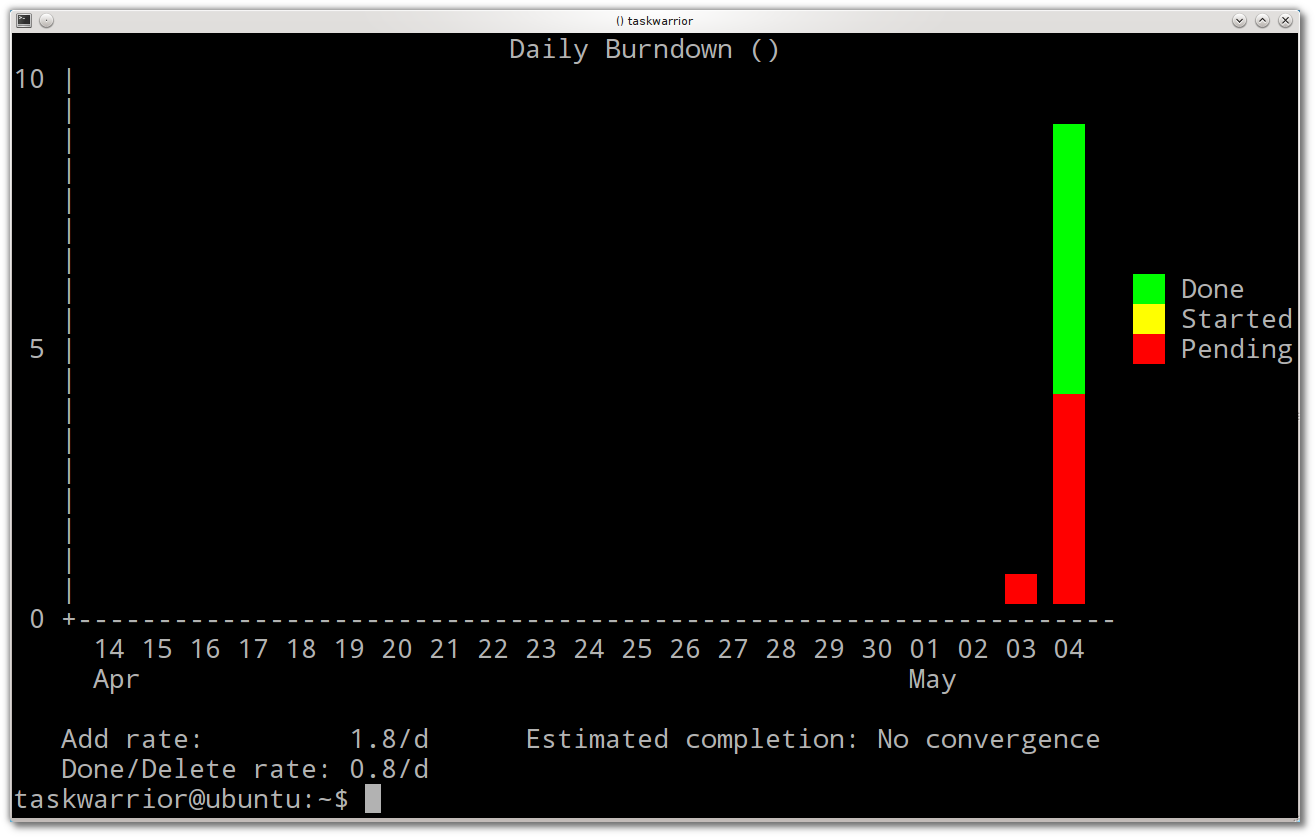
\includegraphics[width=11.8cm,height=7.5cm]{burndown-daily.png}
\end{center}
%\begin{lstlisting}
%task burndown.daily
%\end{lstlisting}
\end{frame}

\begin{frame}[fragile]\frametitle{ghistory, history}
\begin{center} % 1316x838
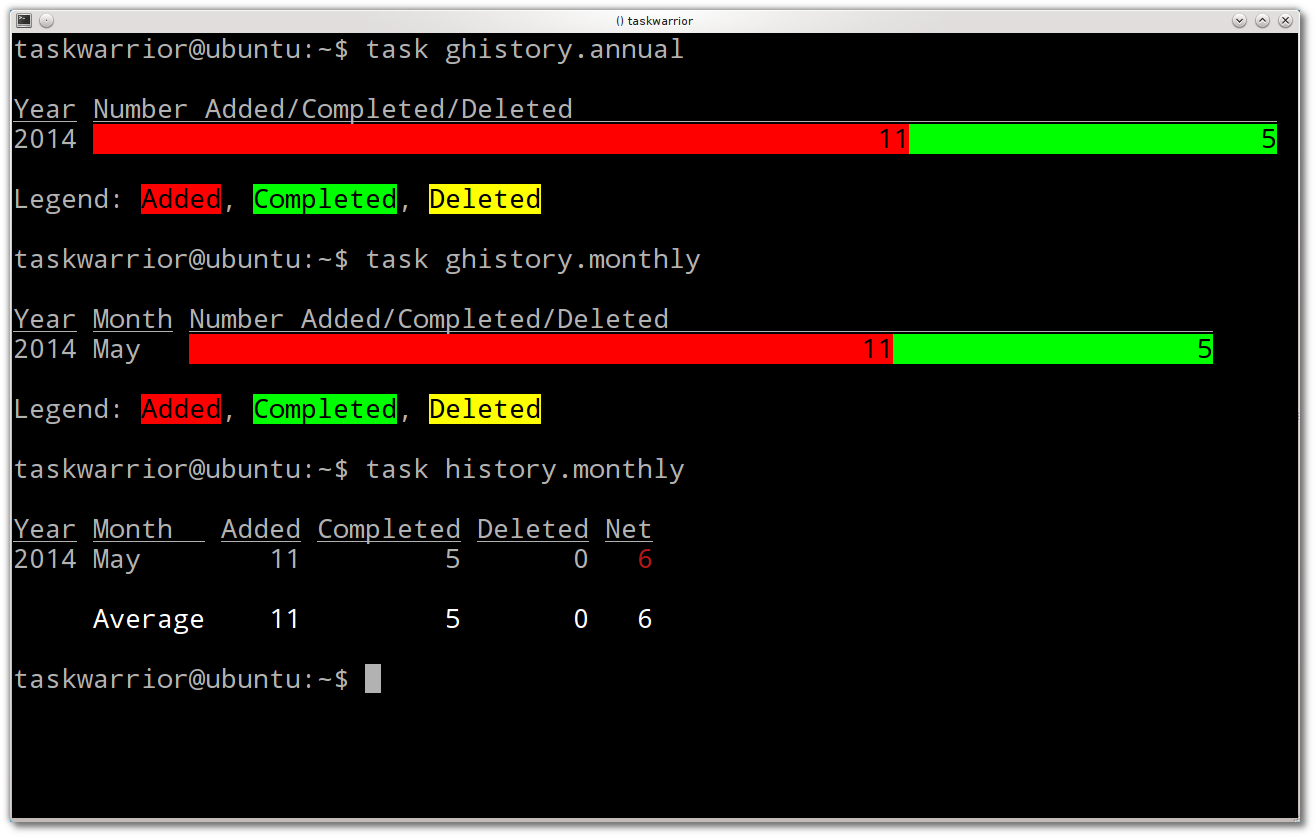
\includegraphics[width=11.8cm,height=7.5cm]{ghistory-history.png}
\end{center}
%\begin{lstlisting}
%task ghistory.annual
%task ghistory.monthly
%task history.monthly
%\end{lstlisting}
\end{frame}

\begin{frame}[fragile]\frametitle{ls, minimal, summary}
\begin{center} % 1316x838
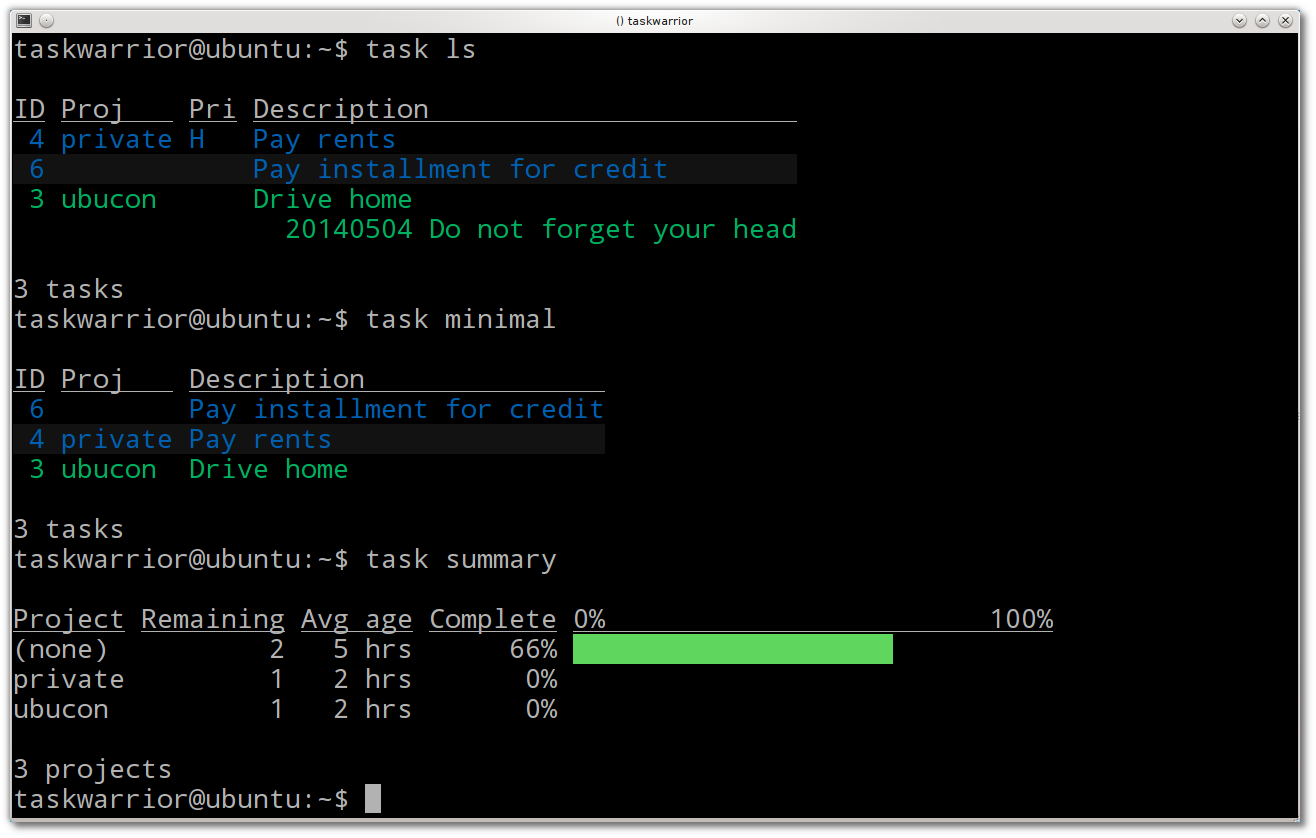
\includegraphics[width=11.8cm,height=7.5cm]{ls-minimal-summary.png}
\end{center}
%\begin{lstlisting}
%task ls
%task minimal
%task summary
%\end{lstlisting}
\end{frame}

\begin{frame}[fragile]\frametitle{Report definitions}
\begin{center} % 1316x838
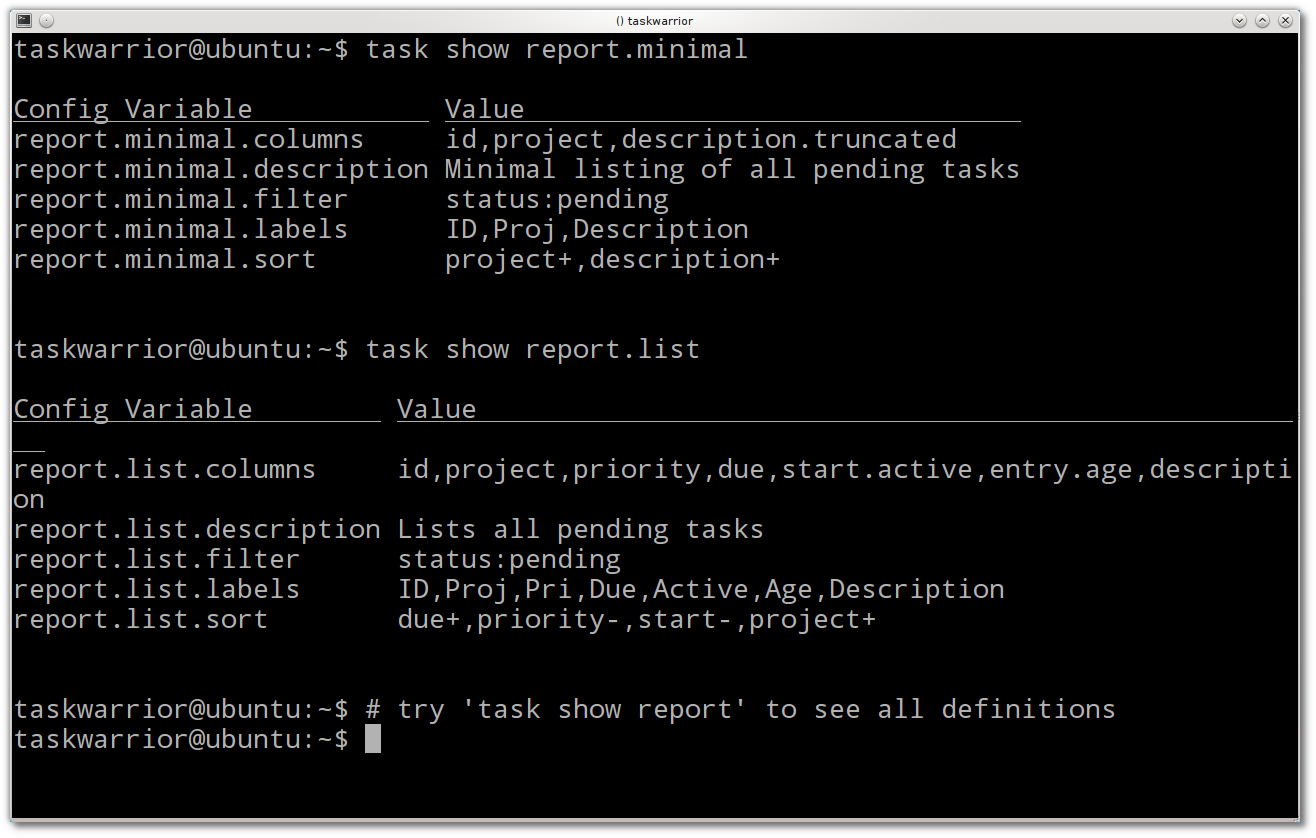
\includegraphics[width=11.8cm,height=7.5cm]{report-definitions.png}
\end{center}
%\begin{lstlisting}
%task show report.minimal
%task show report.list
%# try 'task show report' to see all definitions
%\end{lstlisting}
\end{frame}

\begin{frame}[fragile]\frametitle{Dirks task list}
\begin{center} % 1316x838
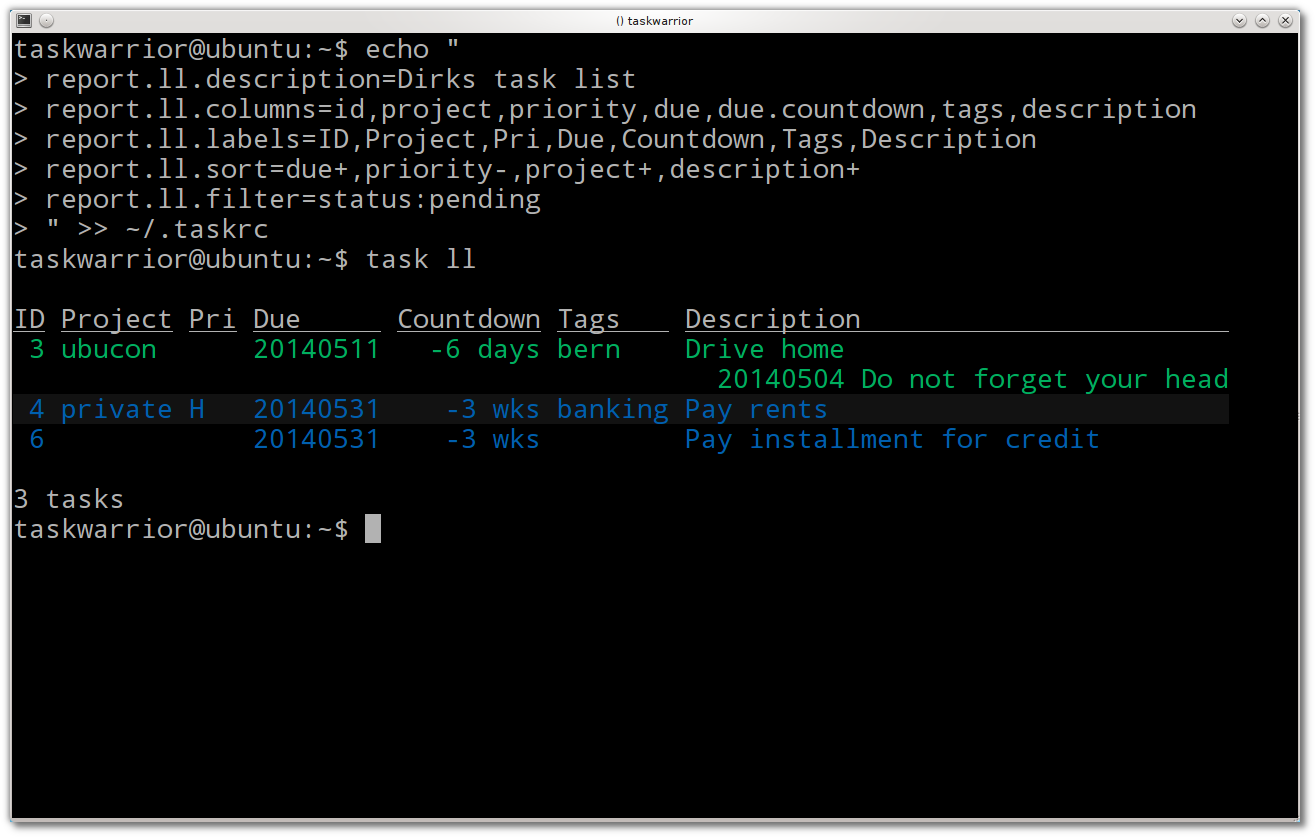
\includegraphics[width=11.8cm,height=7.5cm]{dirks-task-list.png}
\end{center}
%\begin{lstlisting}
%echo "
%report.ll.description=Dirks task list
%report.ll.columns=id,project,priority,due,due.countdown,tags,description
%report.ll.labels=ID,Project,Pri,Due,Countdown,Tags,Description
%report.ll.sort=due+,priority-,project+,description+
%report.ll.filter=status:pending
%" >> ~/.taskrc
%task ll
%\end{lstlisting}
\end{frame}

\begin{frame}[fragile]\frametitle{Set default command}
\begin{center} % 1316x838
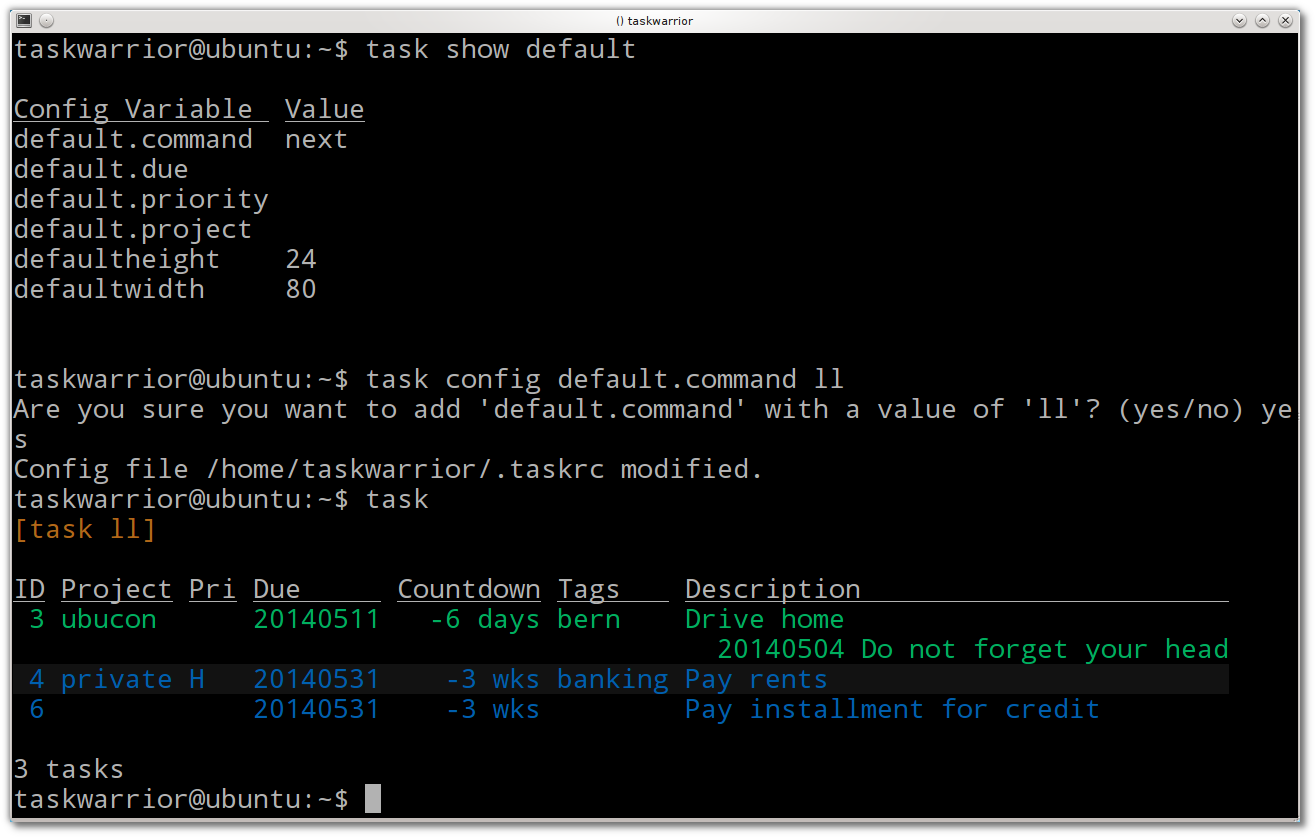
\includegraphics[width=11.8cm,height=7.5cm]{set-default-command.png}
\end{center}
%\begin{lstlisting}
%task show default
%task config default.command ll
%task
%\end{lstlisting}
\end{frame}

%%%%%%%%%%%%%%%%%%%%%%%%%%%
\section{Filtering}
%%%%%%%%%%%%%%%%%%%%%%%%%%%

\begin{frame}\frametitle{Filtering in general}

You can filter for any modifier. If you don't use a modifier description is searched for the term, which may be a regular expression, on the command line. Filters may be combined.

The following attribute modifiers maybe applied as well. Names in brackets can be used alternatively.

So a filter can look like "'attribute.modifier:value"'.

\begin{itemize}
\item before, after
\item none, any
\item is (equals), isnt (not)
\item has (contains), hasnt
\item startswith (left), endswith (right)
\item word, noword
\end{itemize}
\end{frame}

\begin{frame}[fragile]\frametitle{Searches}
\begin{center} % 1316x838
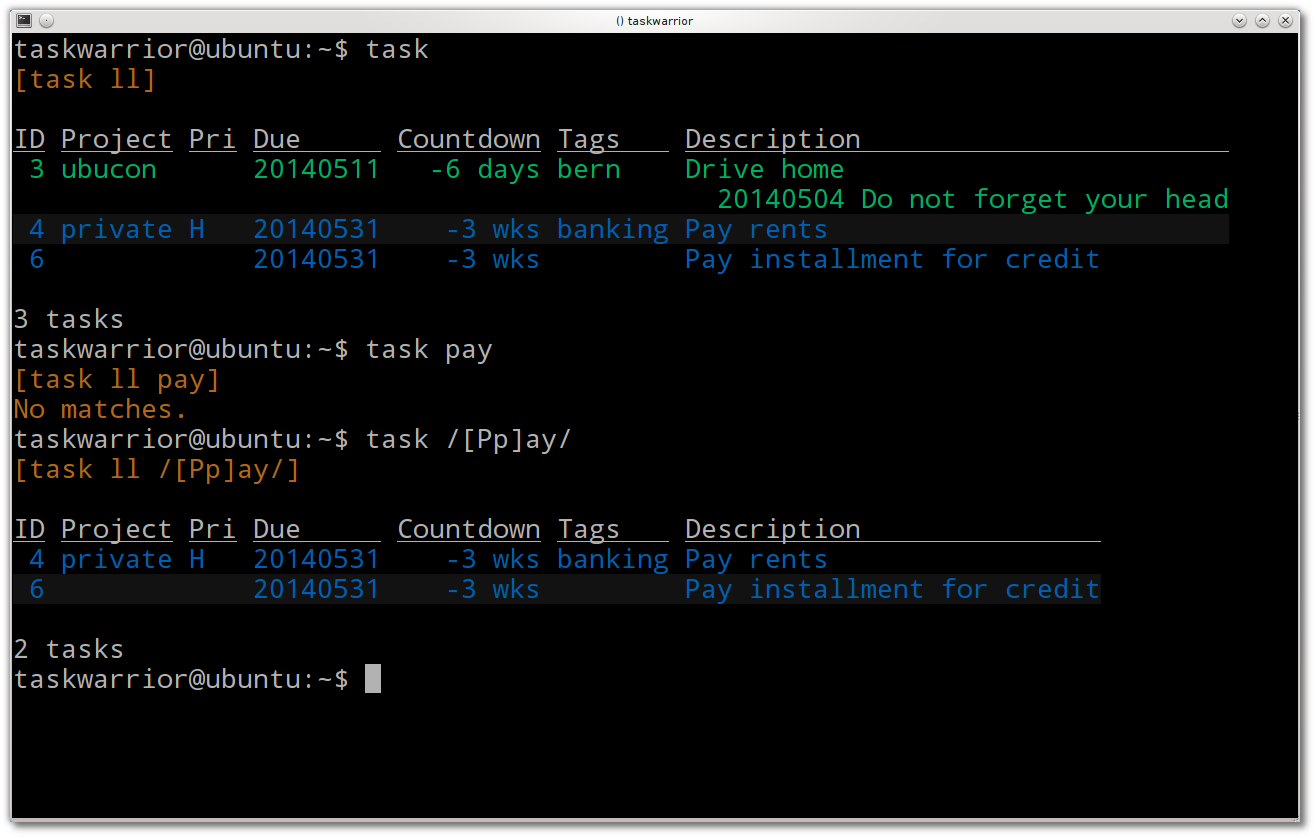
\includegraphics[width=11.8cm,height=7.5cm]{searches.png}
\end{center}
%\begin{lstlisting}
%task
%task pay
%task /[Pp]ay/
%\end{lstlisting}
\end{frame}

\begin{frame}[fragile]\frametitle{Attribute modifiers}
\begin{center} % 1316x838
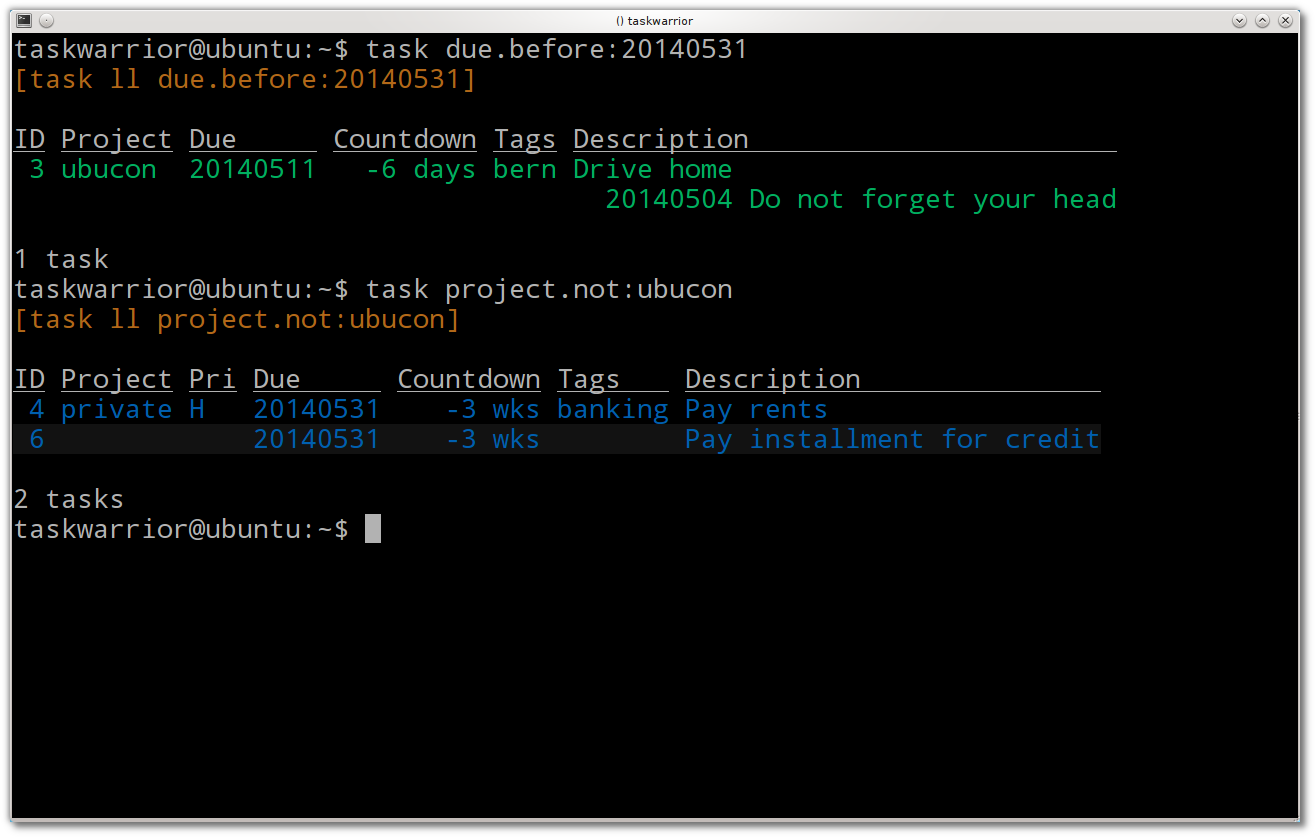
\includegraphics[width=11.8cm,height=7.5cm]{attribute-modifiers.png}
\end{center}
%\begin{lstlisting}
%task due.before:20140531
%task project.not:ubucon
%\end{lstlisting}
\end{frame}

\begin{frame}[fragile]\frametitle{Combining}
\begin{center} % 1316x838
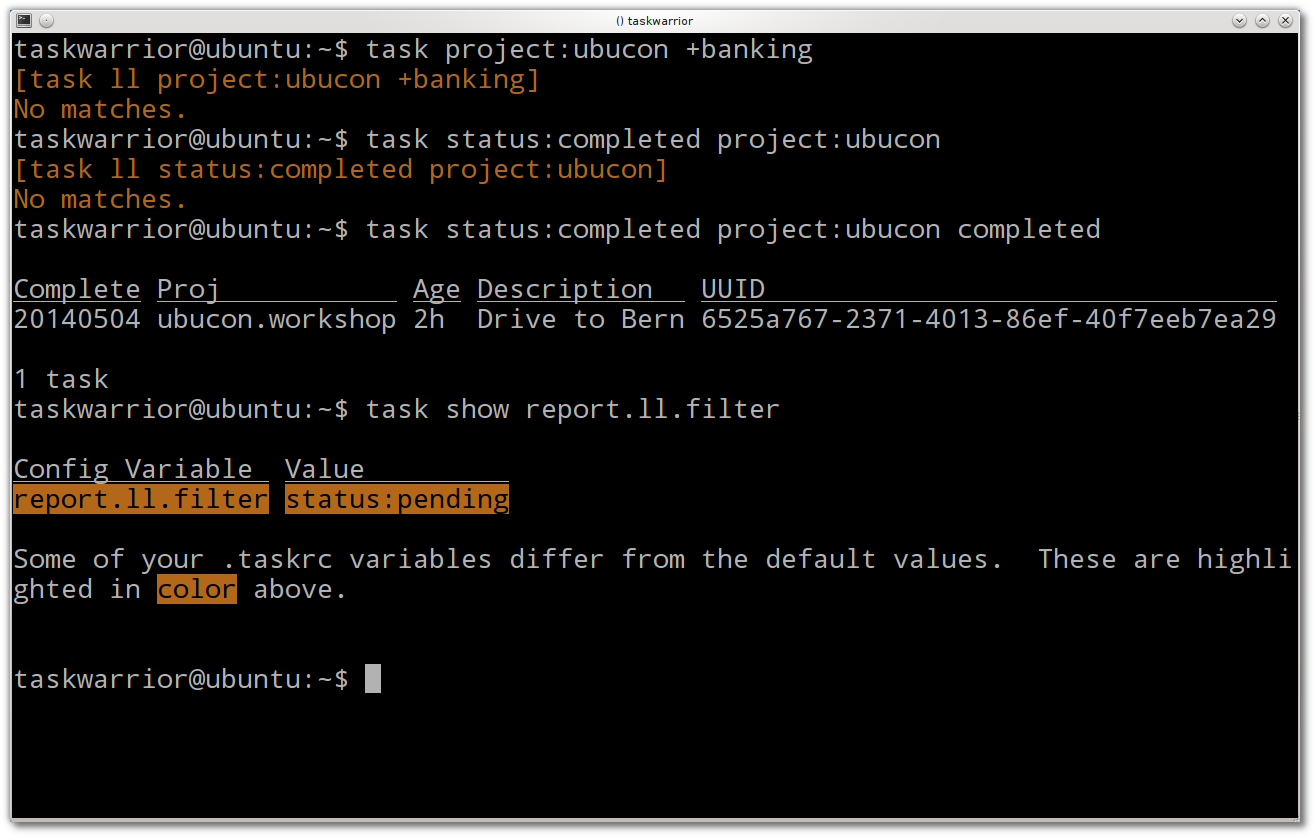
\includegraphics[width=11.8cm,height=7.5cm]{combining.png}
\end{center}
%\begin{lstlisting}
%task project:ubucon +banking
%task status:completed project:ubucon
%task status:completed project:ubucon completed
%task show report.ll.filter
%\end{lstlisting}
\end{frame}

\begin{frame}[fragile]\frametitle{Or ...}
\begin{center} % 1316x838
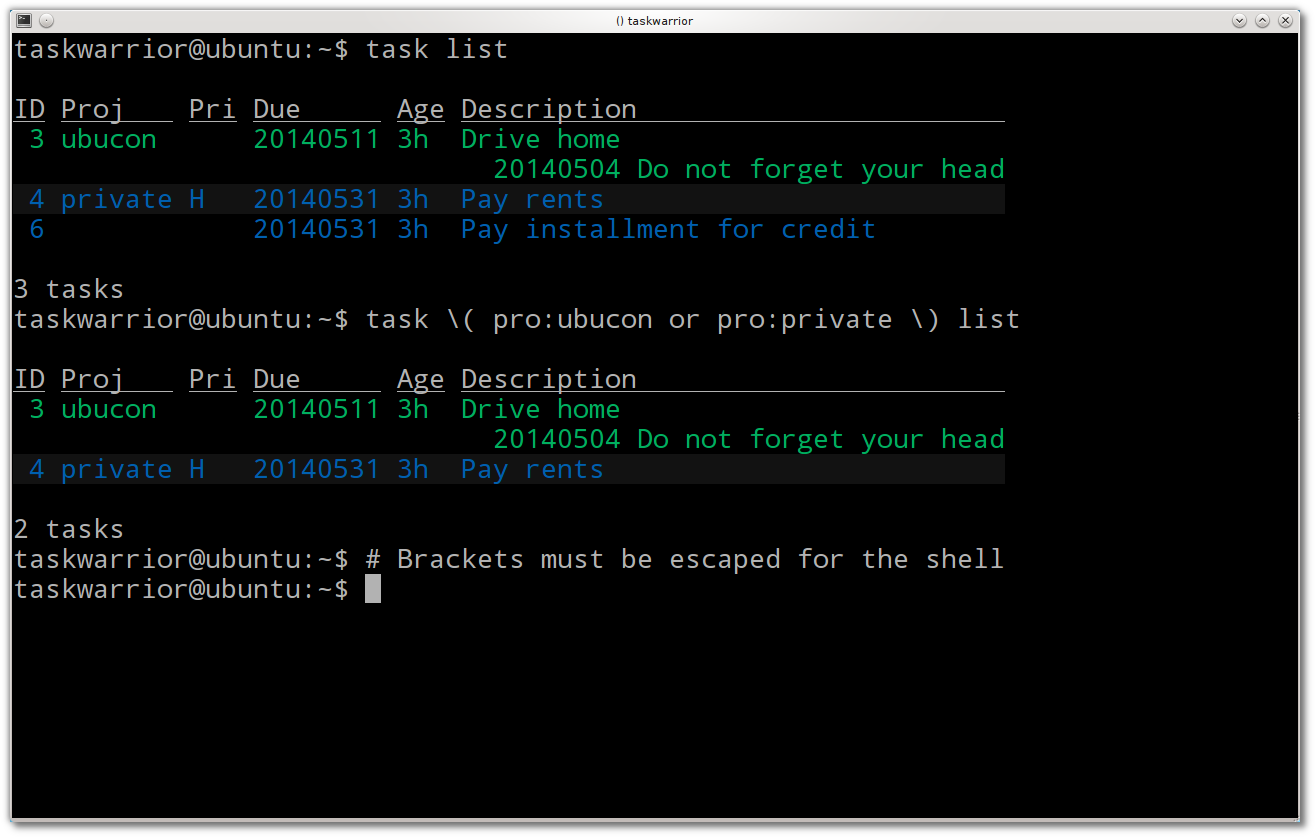
\includegraphics[width=11.8cm,height=7.5cm]{or.png}
\end{center}
%\begin{lstlisting}
%task list
%task \( pro:ubucon or pro:private \) list
%# Brackets must be escaped for the shell
%\end{lstlisting}
\end{frame}

\begin{frame}[fragile]\frametitle{Search configuration}
\begin{center} % 1316x838
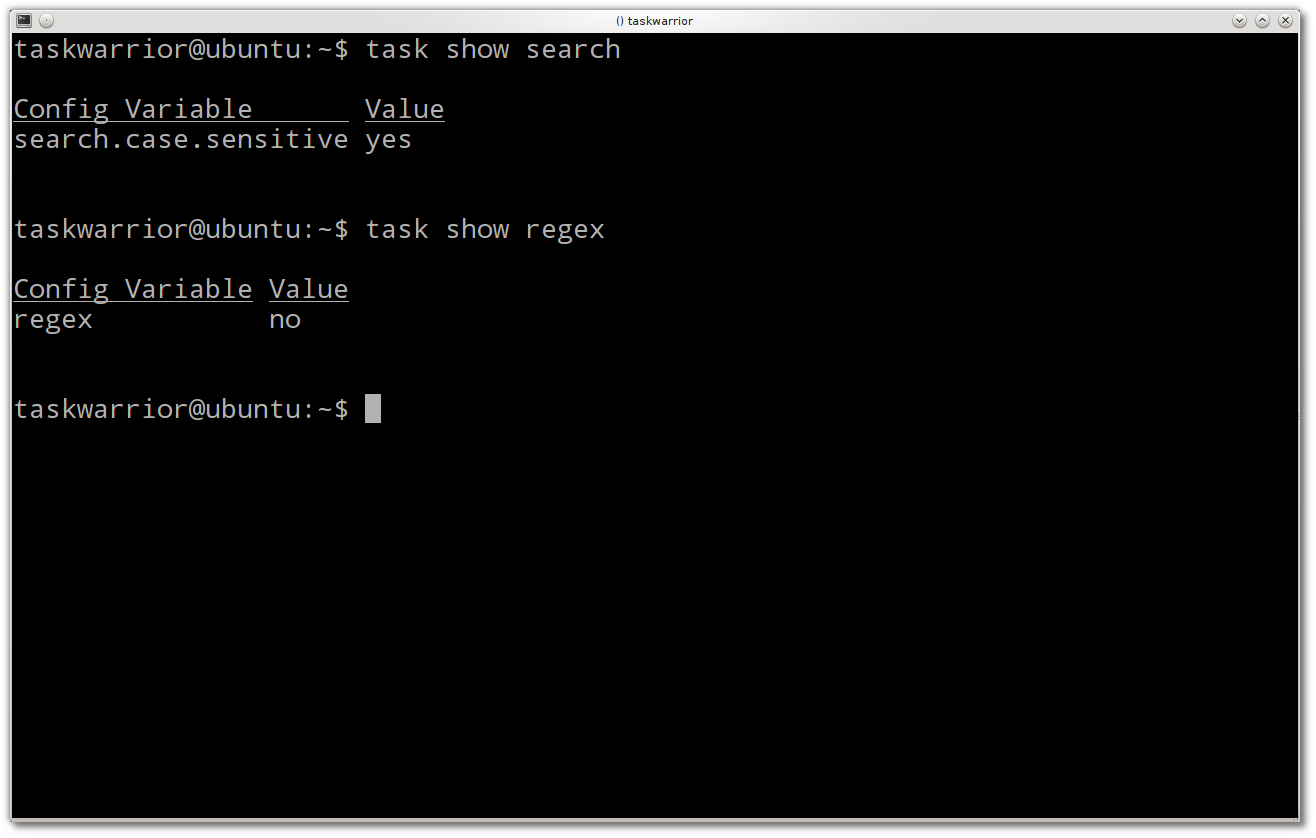
\includegraphics[width=11.8cm,height=7.5cm]{search-configuration.png}
\end{center}
%\begin{lstlisting}
%task show search
%task show regex
%\end{lstlisting}
\end{frame}

\begin{frame}[fragile]\frametitle{Filter in reports}
\begin{center} % 1316x838
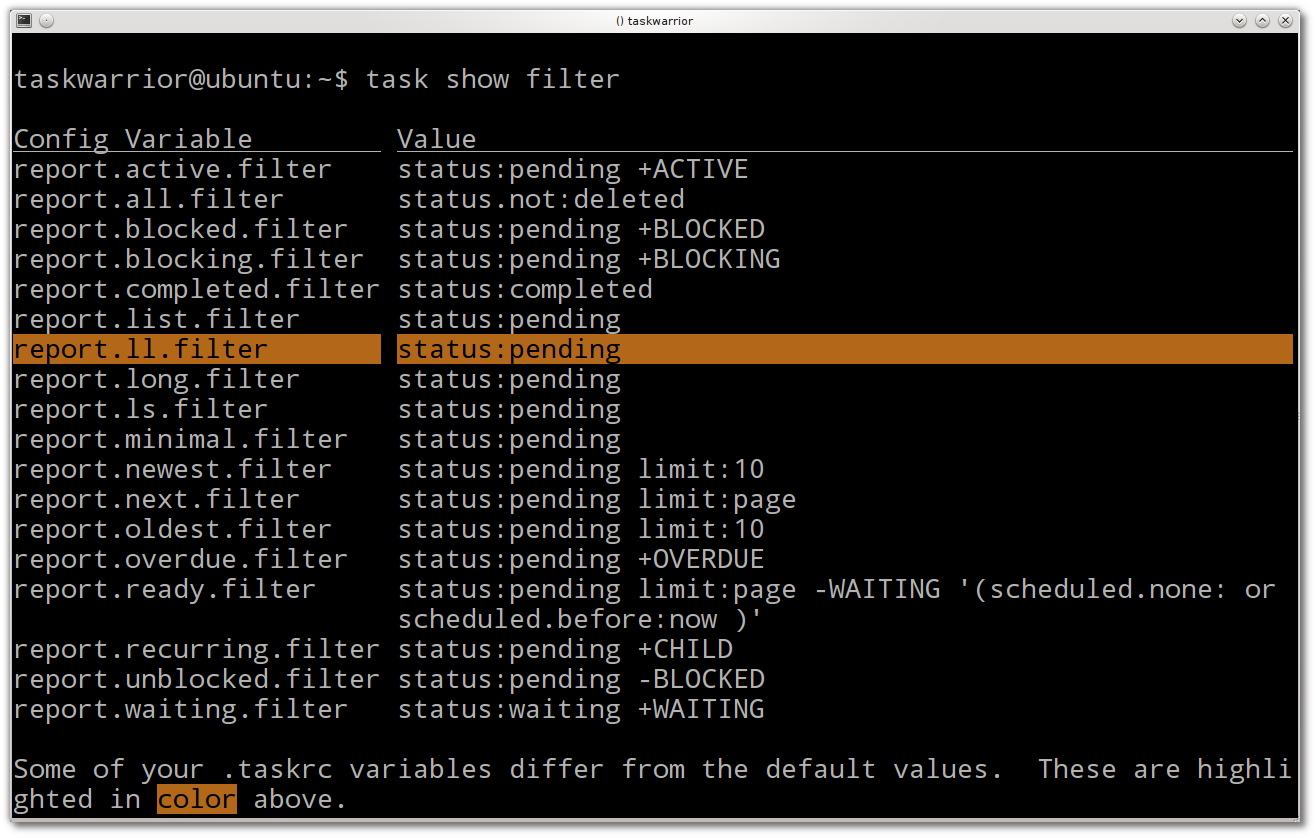
\includegraphics[width=11.8cm,height=7.5cm]{filter-in-reports.png}
\end{center}
%\begin{lstlisting}
%task show filter
%\end{lstlisting}
\end{frame}

%%%%%%%%%%%%%%%%%%%%%%%%%%%
\section{Miscellanous}
%%%%%%%%%%%%%%%%%%%%%%%%%%%

\begin{frame}\frametitle{This is by far not all}
\begin{itemize}
\item \textbf{task log}  \\
for logging a task after it is already done.
\item \textbf{task diag} \\
to help support for diagnostic purpose.
\item \textbf{task shell} \\
a simple shell to get rid of the necessity to type "'task"' all the time.
\item ... and many more!
\end{itemize}
\end{frame}

\begin{frame}\frametitle{Questions?}
\begin{center}

\includegraphics[width=6.4cm,height=7.5cm]{task_logo.png}
\end{center}
\end{frame}

%%%%%%%%%%%%%%%%%%%%%%%%%%%
\section{Ressources} 
%%%%%%%%%%%%%%%%%%%%%%%%%%%

\begin{frame}\frametitle{Support}
\begin{center}
\href{https://answers.tasktools.org/}{answers.tasktools.org}

\href{mailto:support@taskwarrior.org}{support@taskwarrior.org}

\#taskwarrior on freenode.net

@taskwarrior on Twitter or identi.ca
\end{center}
\end{frame}

\begin{frame}\frametitle{taskwarrior.org -- main page}
\begin{center}
\href{http://taskwarrior.org}{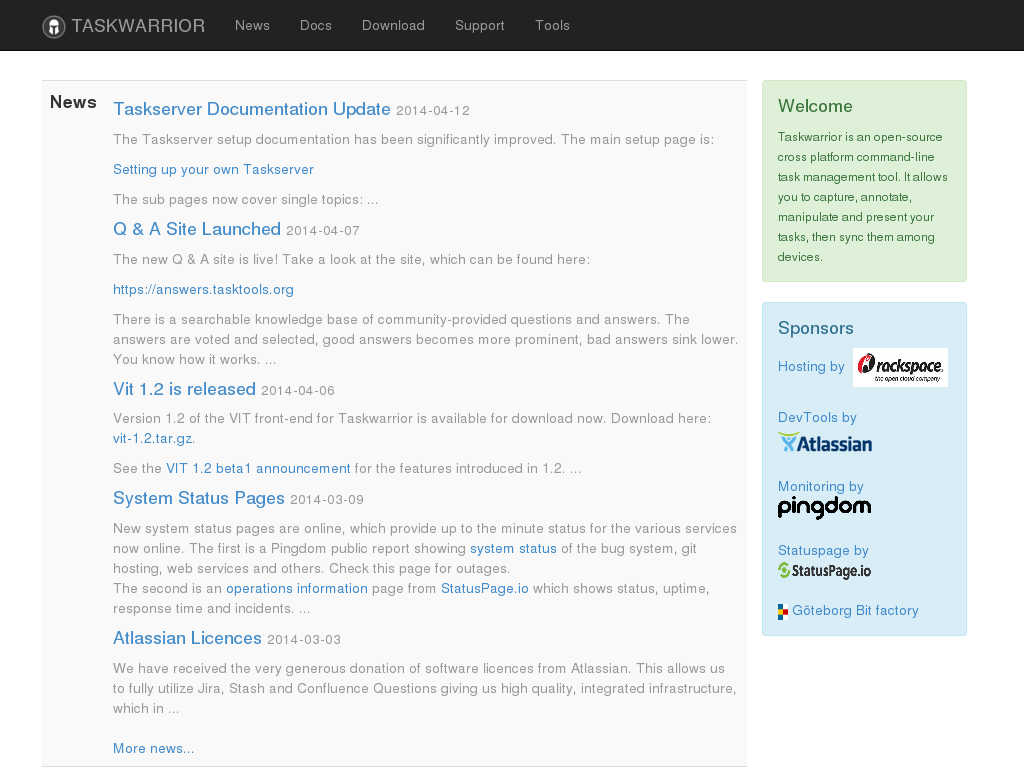
\includegraphics[width=10cm,height=7.5cm]{taskwarrior-org.png}}
\end{center}
\end{frame}

\begin{frame}\frametitle{answers.tasktools.org -- Questions and answers}
\begin{center}
\href{http://answers.tasktools.org/}{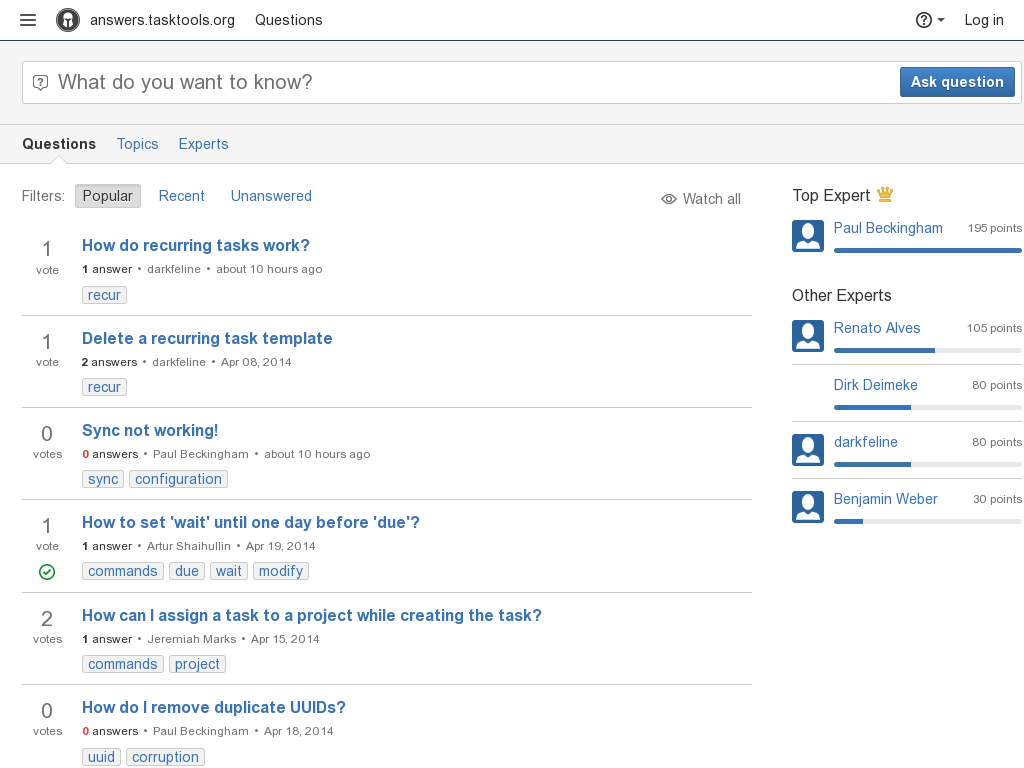
\includegraphics[width=10cm,height=7.5cm]{answers-tasktools-org.png}}
\end{center}
\end{frame}

\begin{frame}\frametitle{status.tasktools.org -- status of the universe}
\begin{center}
\href{http://status.tasktools.org/}{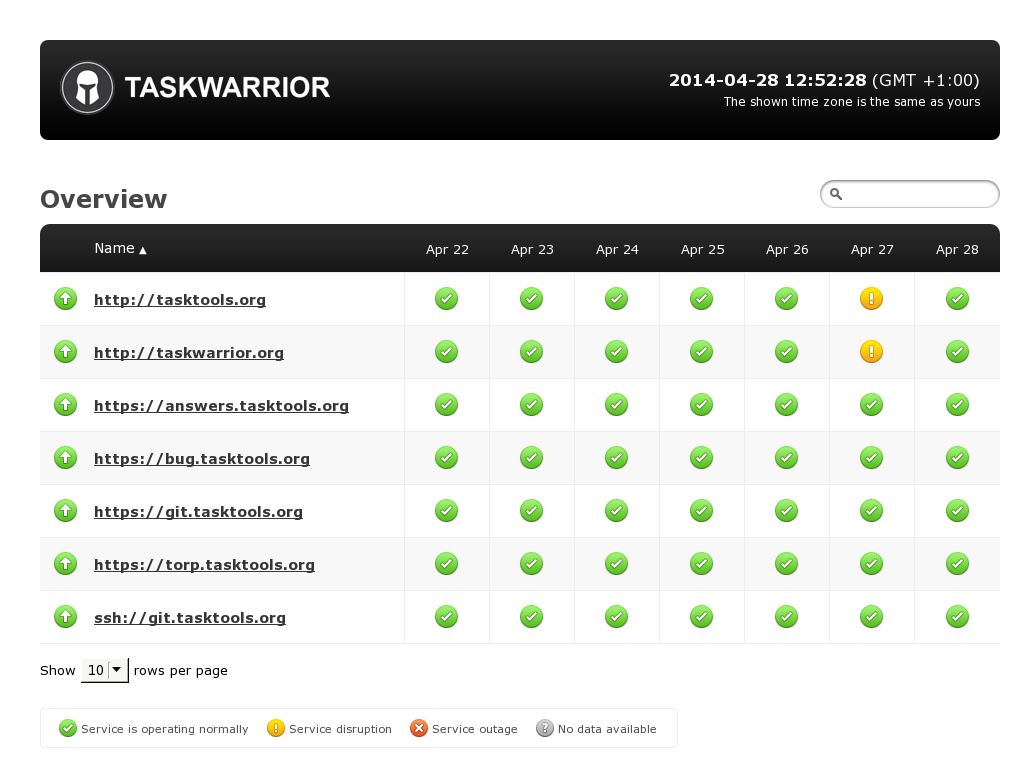
\includegraphics[width=10cm,height=7.5cm]{status-tasktools-org.png}}
\end{center}
\end{frame}

\begin{frame}\frametitle{statuspage.tasktools.org -- more status}
\begin{center}
\href{http://statuspage.tasktools.org/}{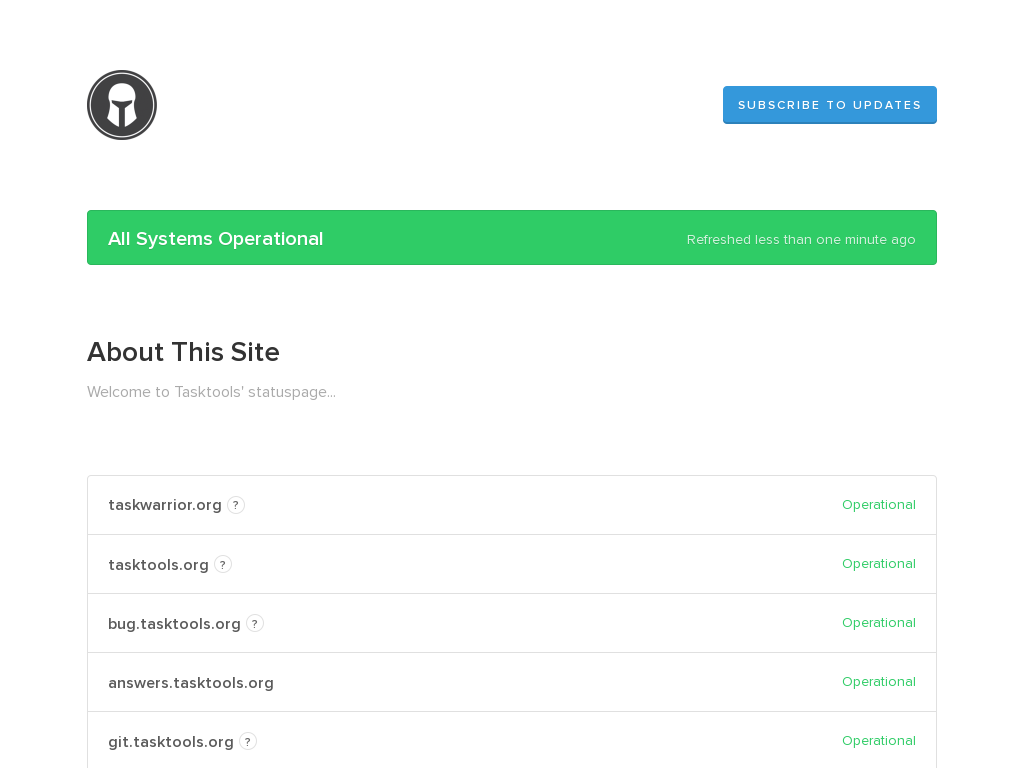
\includegraphics[width=10cm,height=7.5cm]{statuspage-tasktools-org.png}}
\end{center}
\end{frame}

\begin{frame}\frametitle{bug.tasktools.org -- issue tracking}
\begin{center}
\href{https://bug.tasktools.org/}{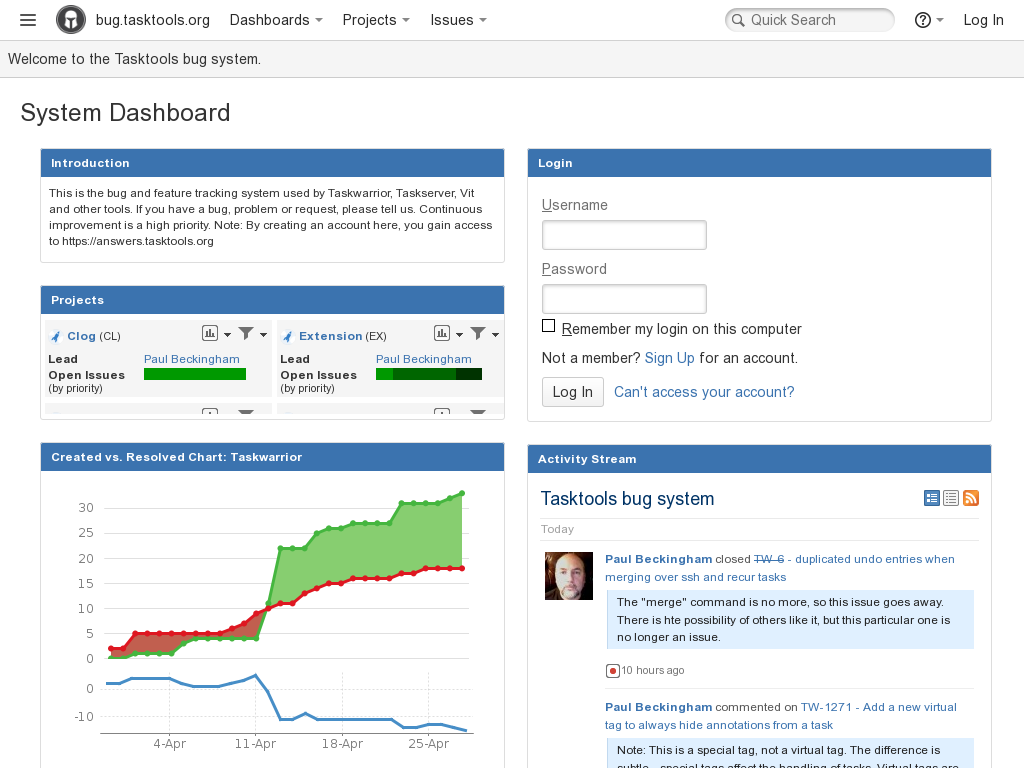
\includegraphics[width=10cm,height=7.5cm]{bug-tasktools-org.png}}
\end{center}
\end{frame}

\begin{frame}\frametitle{git.tasktools.org -- repository management}
\begin{center}
\href{https://git.tasktools.org/}{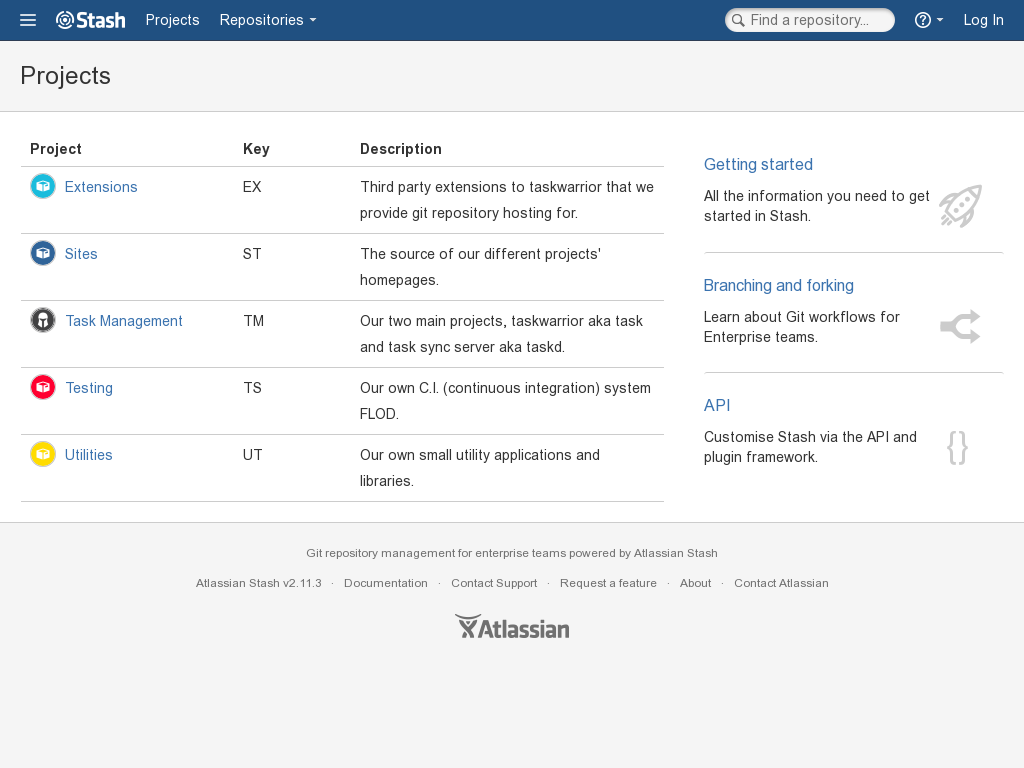
\includegraphics[width=10cm,height=7.5cm]{git-tasktools-org.png}}
\end{center}
\end{frame}

\begin{frame}\frametitle{tasktools.org -- collection of software}
\begin{center}
\href{http://tasktools.org/}{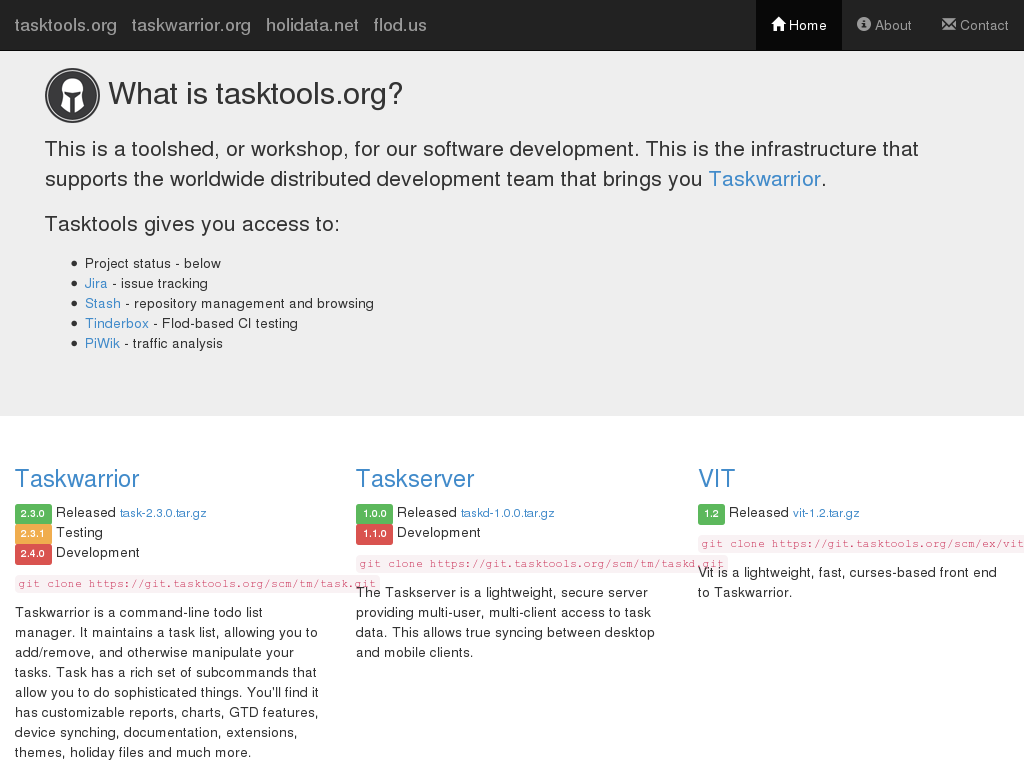
\includegraphics[width=10cm,height=7.5cm]{tasktools-org.png}}
\end{center}
\end{frame}

\begin{frame}\frametitle{tasktools.org/tinderbox -- continous integration}
\begin{center}
\href{http://tasktools.org/tinderbox/}{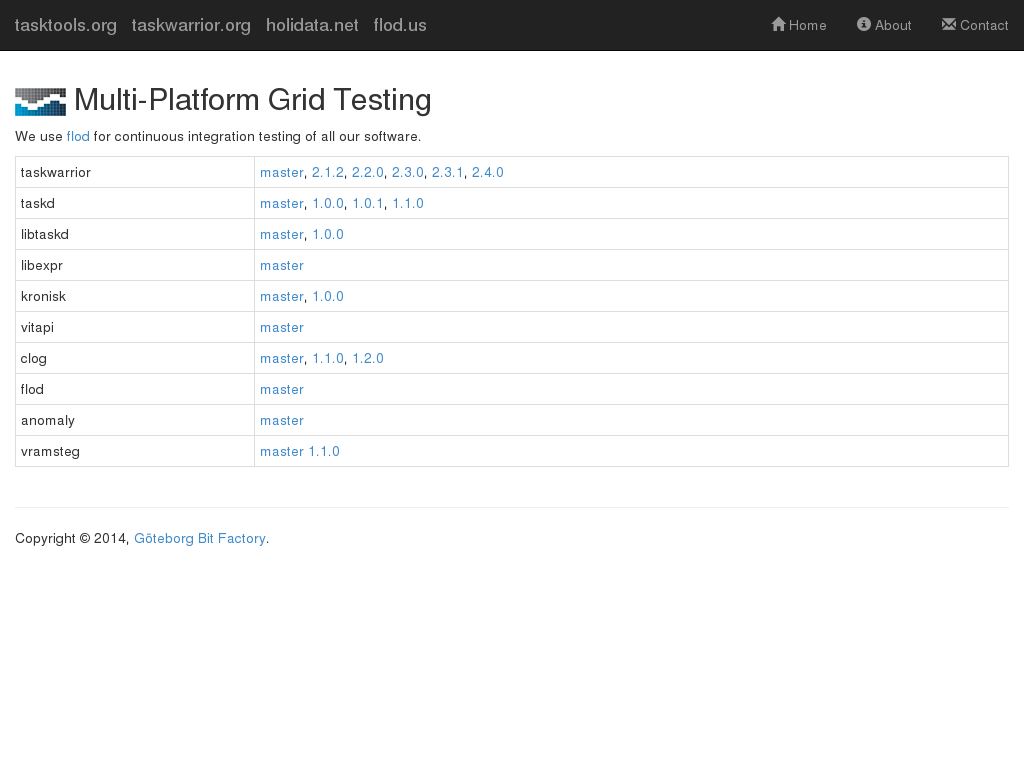
\includegraphics[width=10cm,height=7.5cm]{tasktools-org-tinderbox.png}}
\end{center}
\end{frame}

\begin{frame}\frametitle{holidata.net -- holiday data for several countries}
\begin{center}
\href{http://holidata.net/}{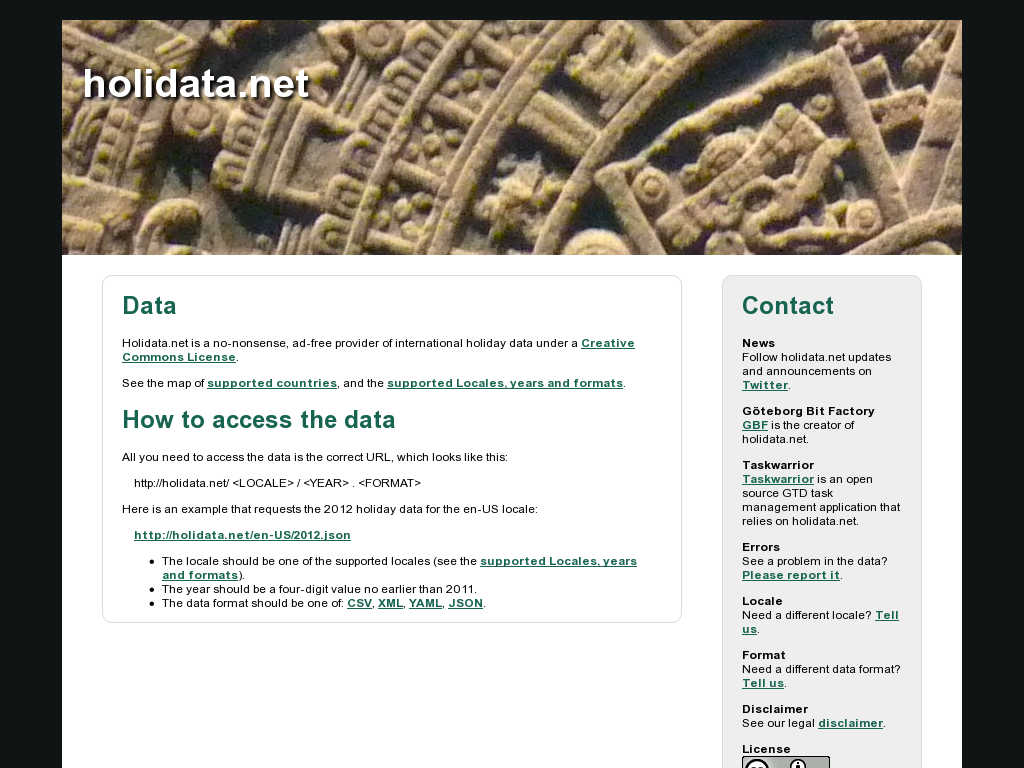
\includegraphics[width=10cm,height=7.5cm]{holidata-net.png}}
\end{center}
\end{frame}

\begin{frame}\frametitle{flod.us -- continous integration framework}
\begin{center}
\href{http://flod.us/}{\includegraphics[width=10cm,height=7.5cm]{flod-us.png}}
\end{center}
\end{frame}

\begin{frame}\frametitle{torp.tasktools.org}
\begin{center}
\href{https://torp.tasktools.org}{\includegraphics[width=10cm,height=7.5cm]{torp-tasktools-org.png}}
\end{center}
\end{frame}

\begin{frame}\frametitle{Thanks for your patience!}
\begin{center}
Dirk Deimeke, Taskwarrior-Team, 2014, \href{https://creativecommons.org/licenses/by/4.0/}{CC-BY}

\href{mailto:dirk@deimeke.net}{dirk@deimeke.net}

\href{http://d5e.org/}{d5e.org} -- \href{http://dirk.deimeke.net/}{dirk.deimeke.net} -- \href{http://deimhart.net/}{deimhart.net}
\end{center}
\end{frame}

\end{document}

% \begin{frame}[fragile]\frametitle{Title}
% \begin{lstlisting}
% \end{lstlisting}
% \end{frame}
% 
% \begin{frame}\frametitle{title}
% \begin{center}
% \includegraphics[width=10cm,height=7.5cm]{name.png}
% \end{center}
% \end{frame}
% 
% \begin{frame}\frametitle{title}
% \begin{itemize}
% \item \textbf{task {\tt<}filter{\tt>} modify}
% \end{itemize}
% \end{frame}
